\documentclass[titlepage,11pt]{article}
\usepackage{comment}
\usepackage{enumitem}
\usepackage{transparent} % Untuk transparansi gambar
\usepackage{listings}
\usepackage{amsmath}
\usepackage{graphicx}
\usepackage[font=small,labelfont=bf]{caption}
\usepackage[bahasa]{babel}
\usepackage{float}
\usepackage{verbatim}
\usepackage{graphicx,tabularx,multirow}
\usepackage{xcolor}
\usepackage[onehalfspacing]{setspace}
\usepackage[
	allcolors=visigrey,
	colorlinks=true,
]{hyperref}
\usepackage[a4paper,left=2cm,right=2cm]{geometry}
% Pengaturan kutipan artikel
\usepackage[style=ieee, backend=biber]{biblatex}
%Code listing style pak akok
\definecolor{codegreen}{rgb}{0,0.6,0}
\definecolor{codegray}{rgb}{0.5,0.5,0.5}
\definecolor{codepurple}{rgb}{0.58,0,0.82}
\definecolor{backcolour}{rgb}{0.95,0.95,0.92}

\usepackage{eso-pic} % Untuk menambahkan elemen ke seluruh halaman

\newcommand\BackgroundPic{
  \put(0,0){
    \parbox[b][\paperheight]{\paperwidth}{
      \vfill
      \centering
      \transparent{0.1}
      \includegraphics[width=0.4\paperwidth,keepaspectratio]{miot.png}
      \vfill
    }
  }
}

\newcommand\BackgroundAllPages{ \AddToShipoutPicture*{\BackgroundPic} }
\newcommand\BackgroundNone{ \ClearShipoutPicture } % hilangkan background

\lstdefinestyle{mystyle}{
	backgroundcolor=\color{backcolour}, commentstyle=\color{codegreen},
	keywordstyle=\color{magenta},
	numberstyle=\small\color{codegray},
	stringstyle=\color{codepurple},
	basicstyle=\ttfamily\footnotesize,
	breakatwhitespace=false,         
	breaklines=true,                 
	captionpos=t,                    
	keepspaces=true,                 
	numbers=left,                    
	numbersep=5pt,                  
	showspaces=false,                
	showstringspaces=false,
	showtabs=false,           
	frame = single,
	tabsize=2
}
\lstset{style=mystyle}

\definecolor{visigrey}{rgb}{.1,.15,.15}
\geometry{top=1cm,bottom=.5cm}
\savegeometry{titlepage}
\geometry{top=2cm,bottom=2cm}
\savegeometry{main}

\def\bspace{\(\qquad\qquad\qquad\)}
\usepackage[T1]{fontenc}
\usepackage[utf8]{inputenc}
\usepackage{tgheros}
\renewcommand*\familydefault{\sfdefault}

\setcounter{tocdepth}{6}

\def\autor{Laboratorium }
\def\lab{Multimedia dan Internet of Things}
\def\departemen{Departemen Teknik Komputer}
\def\institut{Institut Teknologi Sepuluh Nopember}
\def\praktikum{Laporan Sementara \\ Praktikum Jaringan Komputer}
\def\nama{Muhammad Risang Radityatama - 5024231028}
% Ubah Judul sesuai dengan modul
\def\judul{VPN dan QoS}
\def\tanggal{2025}
\begin{document}
% Ubah Bahasa sesuai dengan keinginan
\selectlanguage{bahasa}

\BackgroundNone
\def\headingtype{\bf \small}
\loadgeometry{titlepage}

\begin{titlepage}
	\centering
	\begin{tabularx}{\textwidth}{l@{\hskip 0pt}lX}
		\raisebox{-0.5\height}{
\includegraphics[width=3cm]{Cover/img/logodepart.png}} 
		& \raisebox{-0.5\height}{\includegraphics[width=3cm]{Cover/img/miot.png}} 
		& \raggedleft
	\hfill
	\begin{minipage}{0.5\textwidth}
		\raggedleft
		{\emph{\headingtype \autor}} \\[-2pt]
		{\headingtype \lab} \\[-2pt]
		{\headingtype \departemen} \\[-2pt]
		{\headingtype \emph{\institut}}
	\end{minipage}

	\vspace{5cm}
	\end{tabularx}
	
	\vspace{5cm}
	{\Huge \bf \praktikum \par}
	
	\vspace{2cm}
	{\LARGE \bf \judul \par}
	
	\vspace{2cm}
	{\Large \nama \par}
	
	\vfill
	{\Large \tanggal \par}
	
	\vfill
	
\includegraphics[width=\textwidth]{Cover/img/footer.png}
\end{titlepage}

\loadgeometry{main}


\BackgroundAllPages
% Pilih Modul yang akan di build
\section{Langkah-Langkah Percobaan}
\subsection{VPN PPTP}
\begin{enumerate}
	\item Melakukan reset router bila diperlukan dan login ke router.
	\item Melakukan konfigurasi DHCP client pada interface yang terhubung ke internet (ether7).
	\begin{figure}[H]
		\centering
		\begin{subfigure}[b]{0.4\linewidth}
			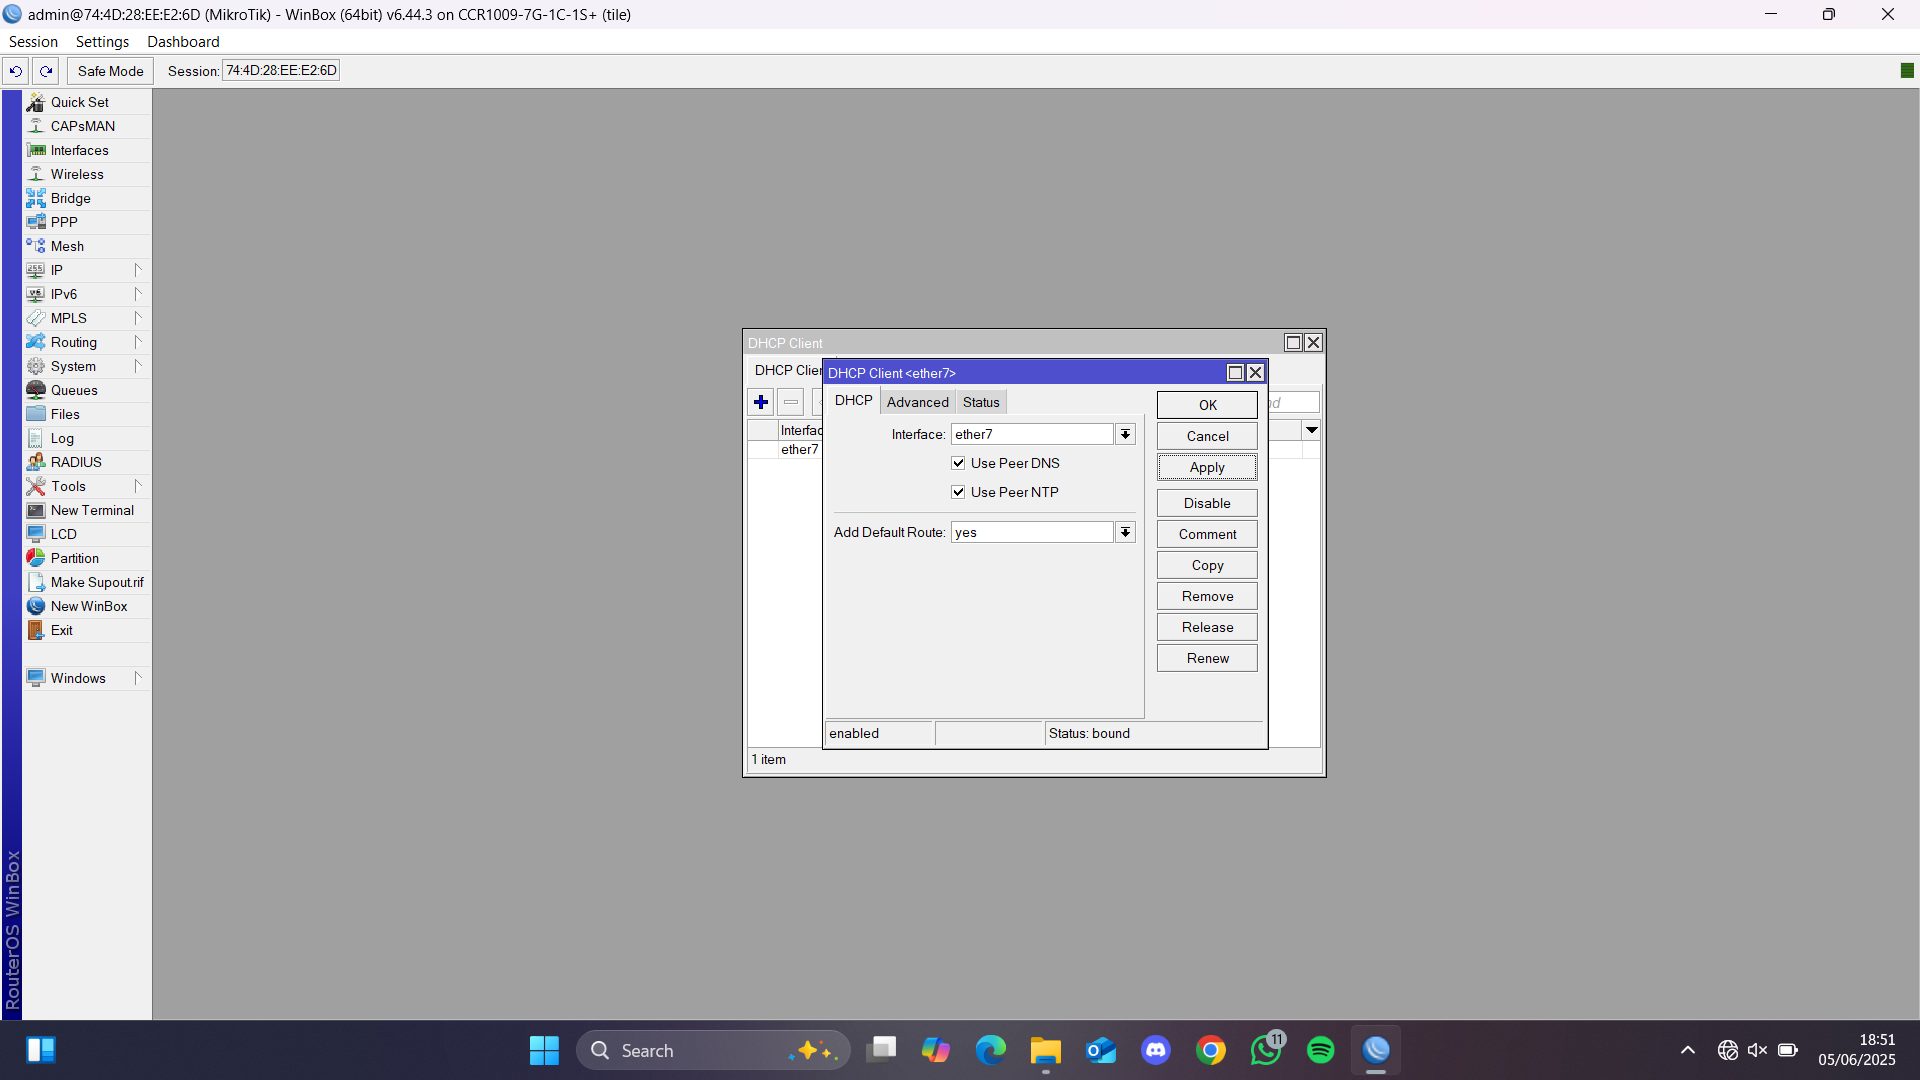
\includegraphics[width=\linewidth]{P5/img/dhcp client.png}
			\caption{Konfigurasi DHCP Client\label{fig:konfigurasiR1}}
		\end{subfigure}
	\end{figure}
	
	\item Melakukan konfigurasi firewall NAT pad interface yang terhubung ke internet. Konfigurasi yang digunakan adalah Chain: src-nat, Out. Interface ether7, Action: masquerade.
	\begin{figure}[H]
		\centering
		\begin{subfigure}[b]{0.4\linewidth}
			\centering
			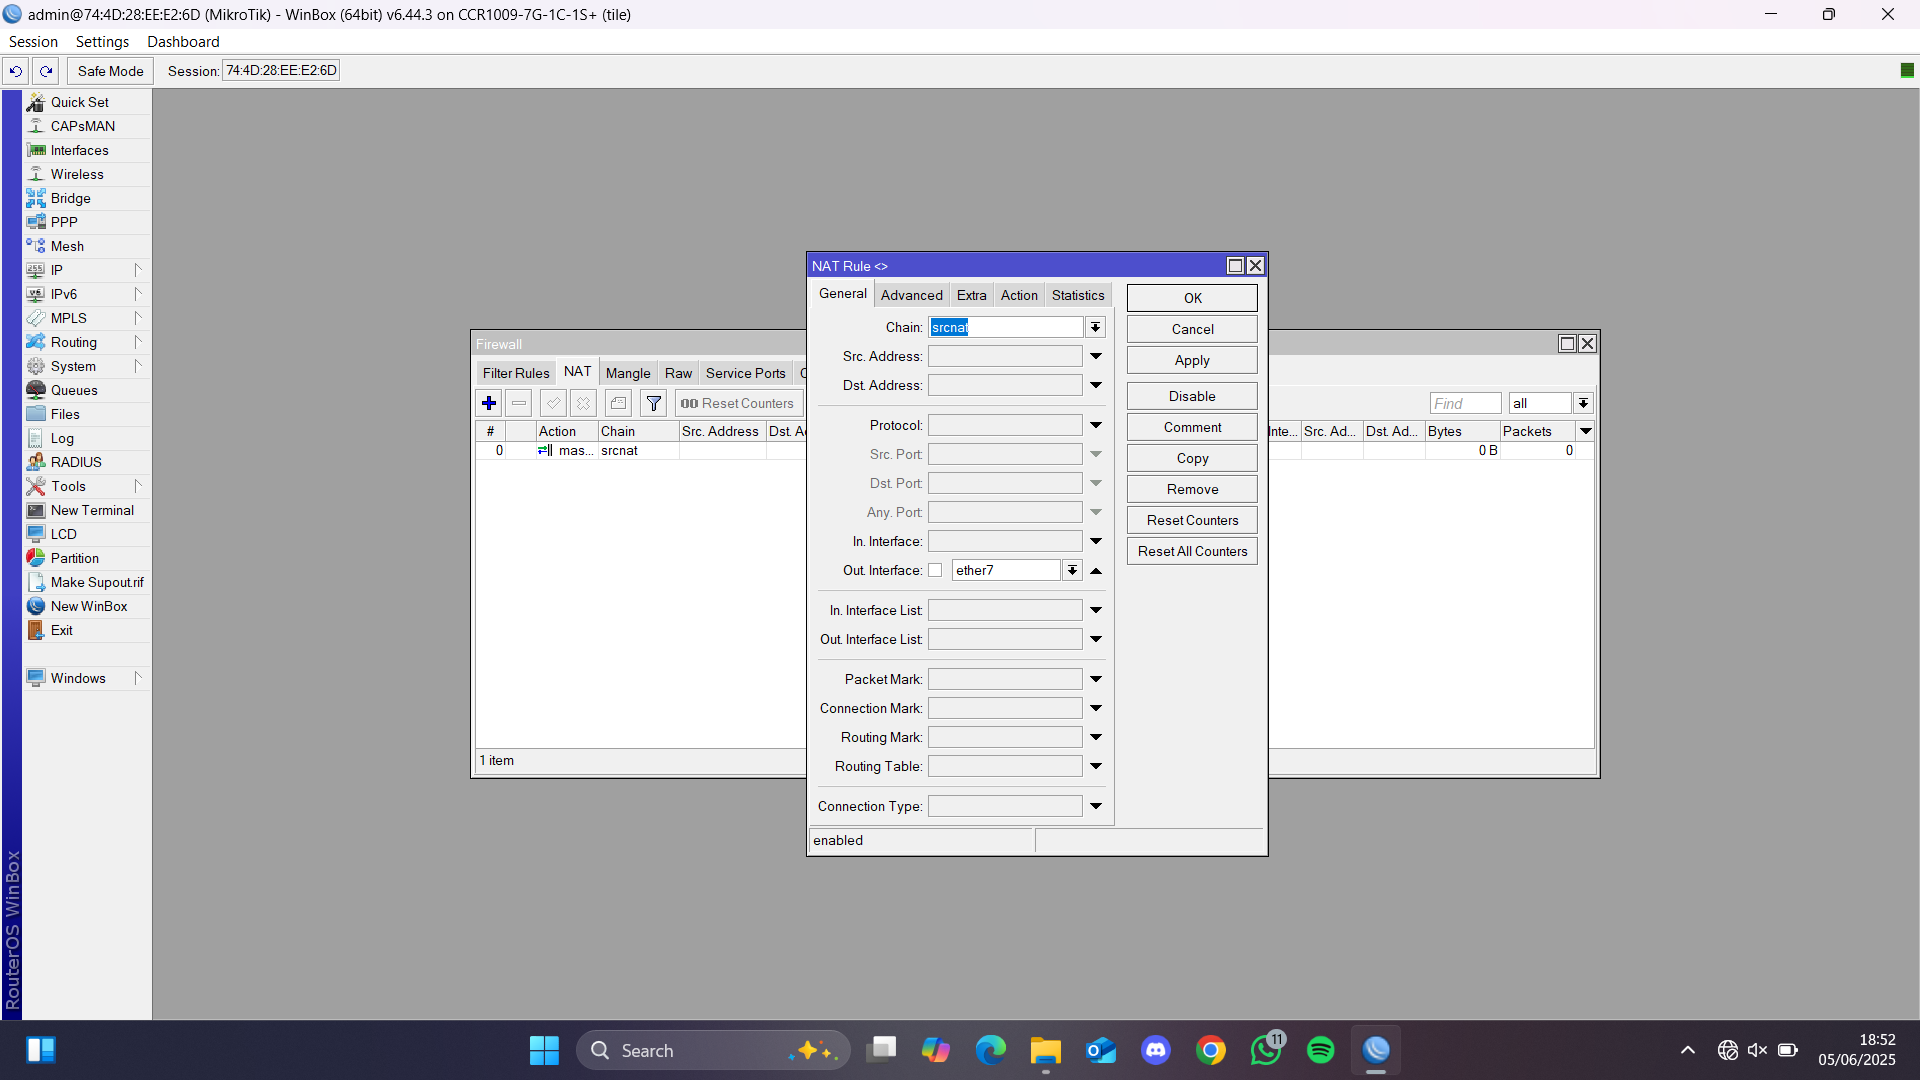
\includegraphics[width=\linewidth]{P5/img/nat (1).png}
			\caption{Konfigurasi chain dan out interface\label{fig:konfigurasiR1}}
		\end{subfigure}
		\begin{subfigure}[b]{0.4\linewidth}
			\centering
			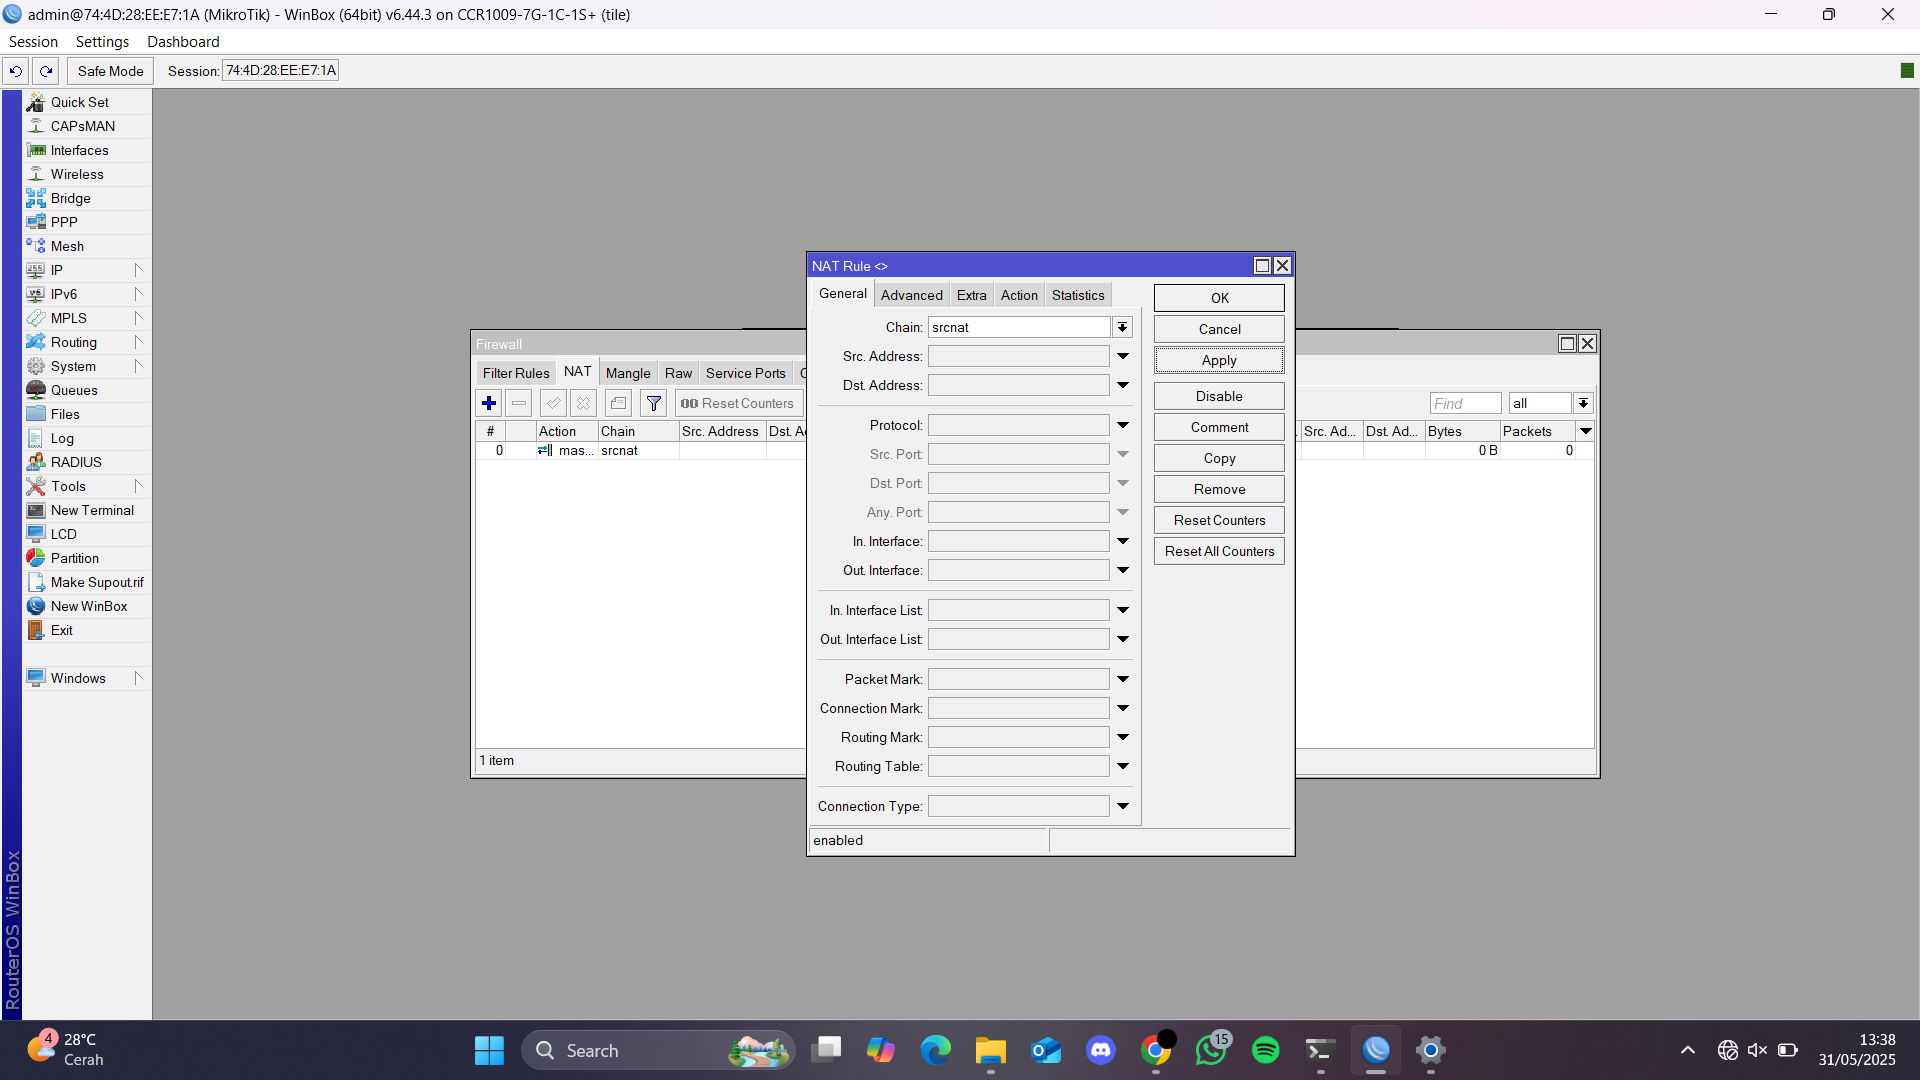
\includegraphics[width=\linewidth]{P5/img/nat (2).png}
			\caption{Konfigurasi action\label{fig:konfigurasiR2}}
		\end{subfigure}
		\caption{Konfigurasi NAT}
		\hspace{1cm}
	\end{figure}
	\item Melakukan konfigurasi alamat IP pada interface yang terhubung ke laptop A, yaitu ether1. Konfigurasi yang digunakan adalah menggunakan address 192.168.10.2/24.
		\begin{figure}[H]
		\centering
		\begin{subfigure}[b]{0.4\linewidth}
			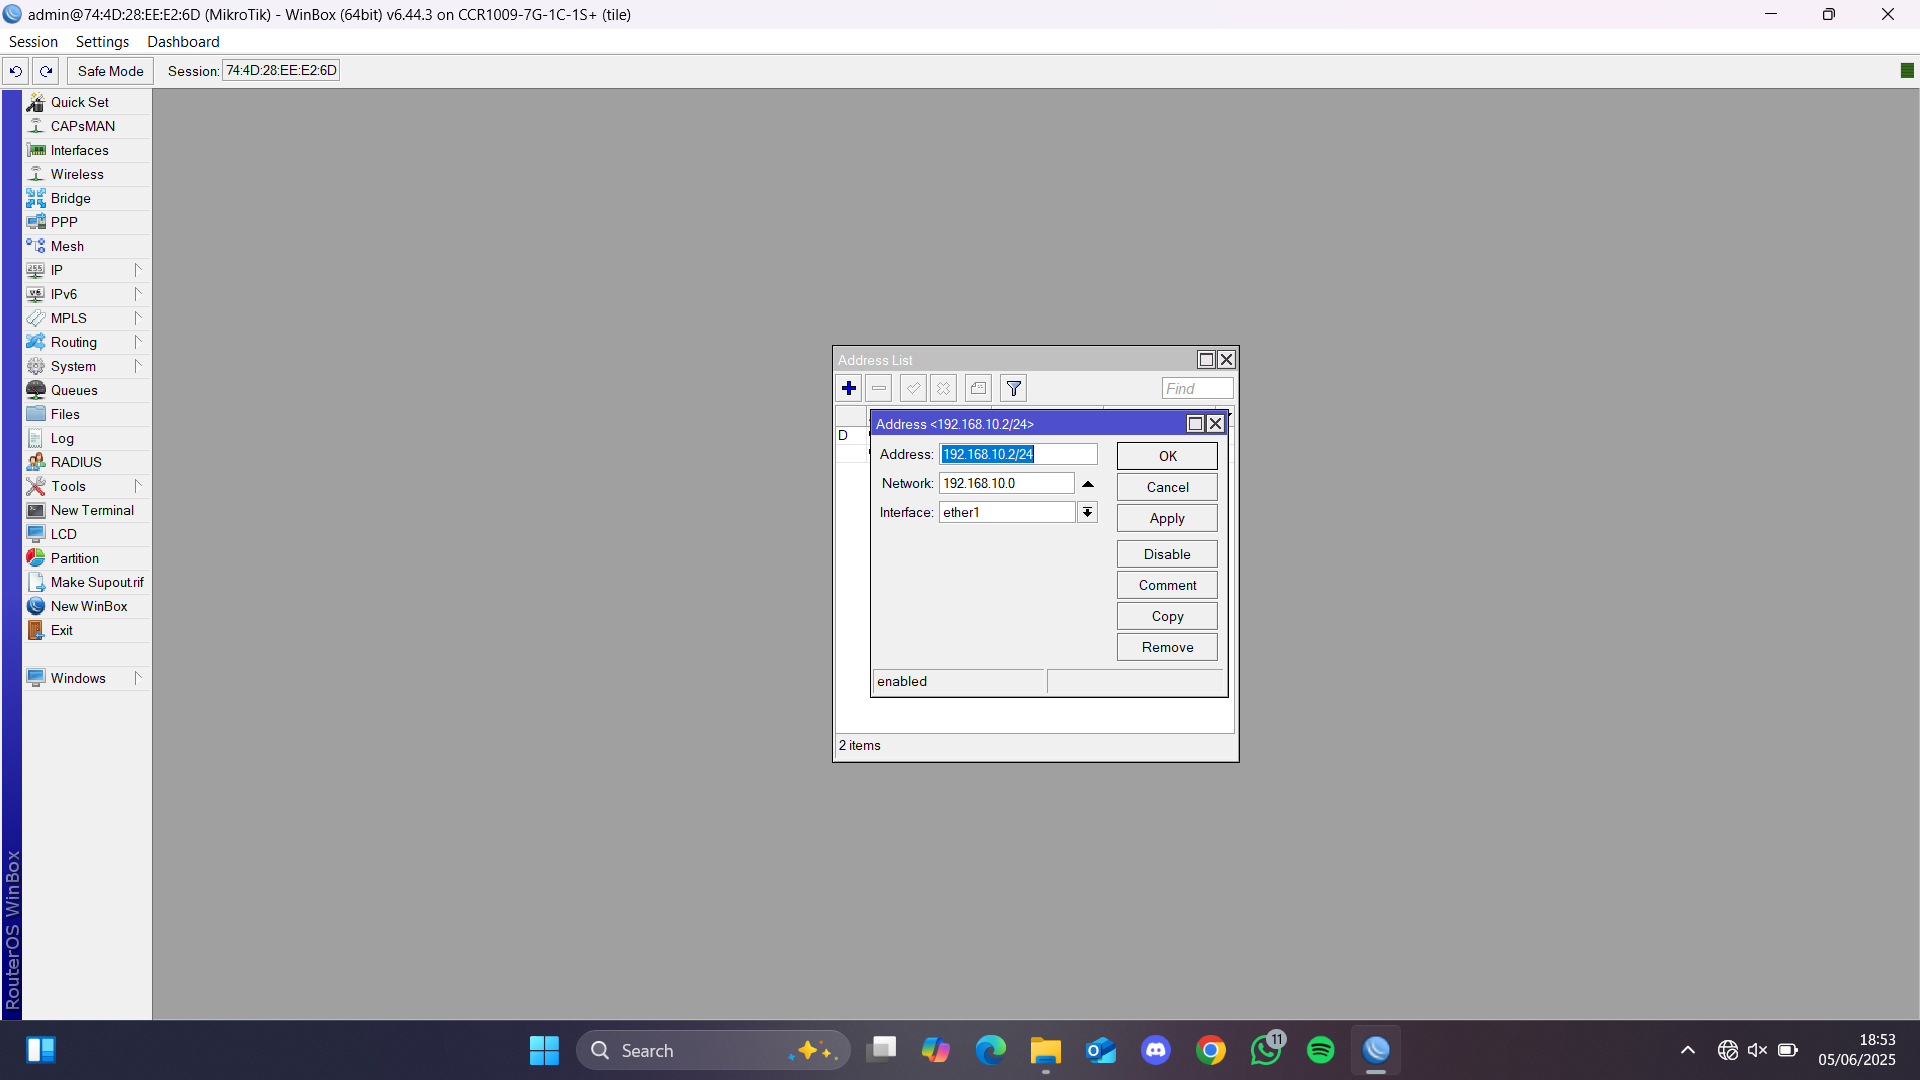
\includegraphics[width=\linewidth]{P5/img/ip conf.png}
			\caption{Konfigurasi IP\label{fig:konfigurasiR1}}
		\end{subfigure}
	\end{figure}
	\item Melakukan setup DHCP server pada interface ether1.
		\begin{figure}[H]
		\centering
		\begin{subfigure}[b]{0.4\linewidth}
			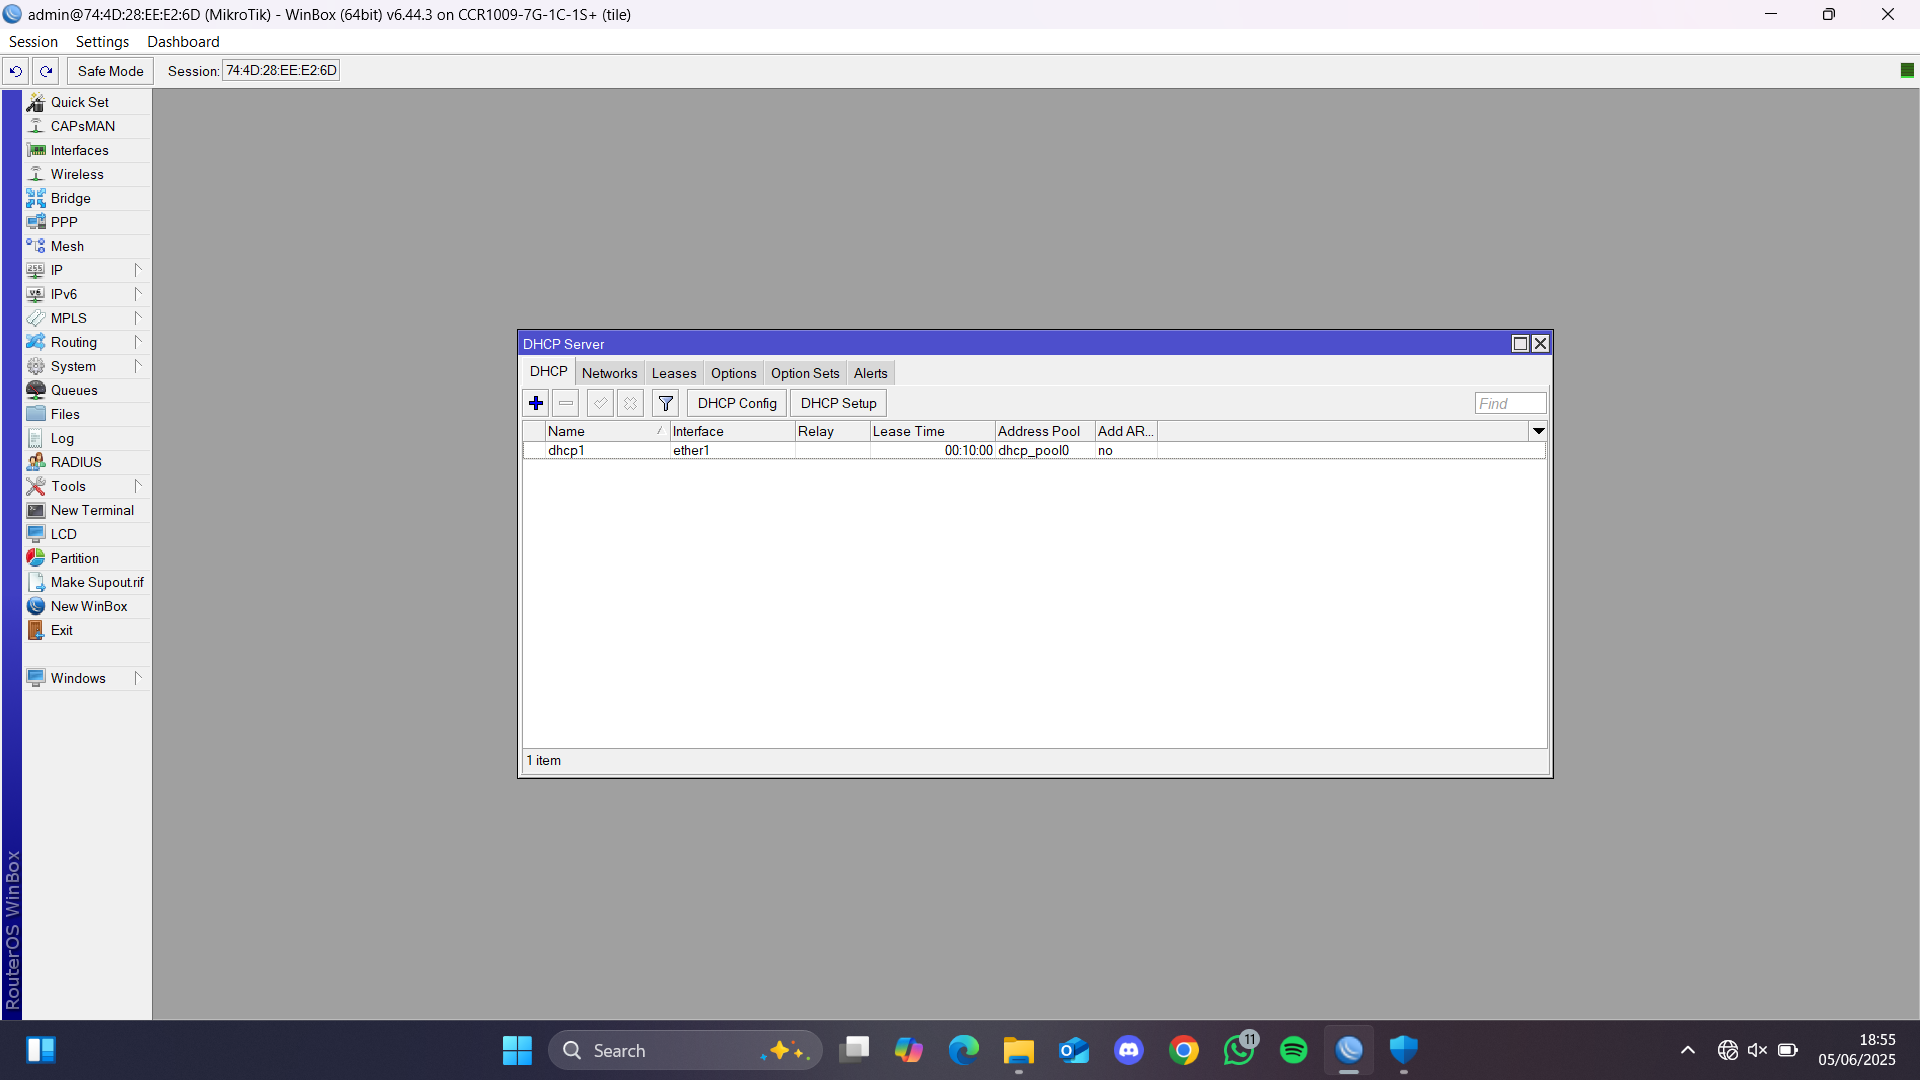
\includegraphics[width=\linewidth]{P5/img/dhcp server.png}
			\caption{Konfigurasi DHCP Server\label{fig:konfigurasiR1}}
		\end{subfigure}
	\end{figure}
	\item Mengaktifkan Proxy ARP pada interface ether1.
		\begin{figure}[H]
		\centering
		\begin{subfigure}[b]{0.4\linewidth}
			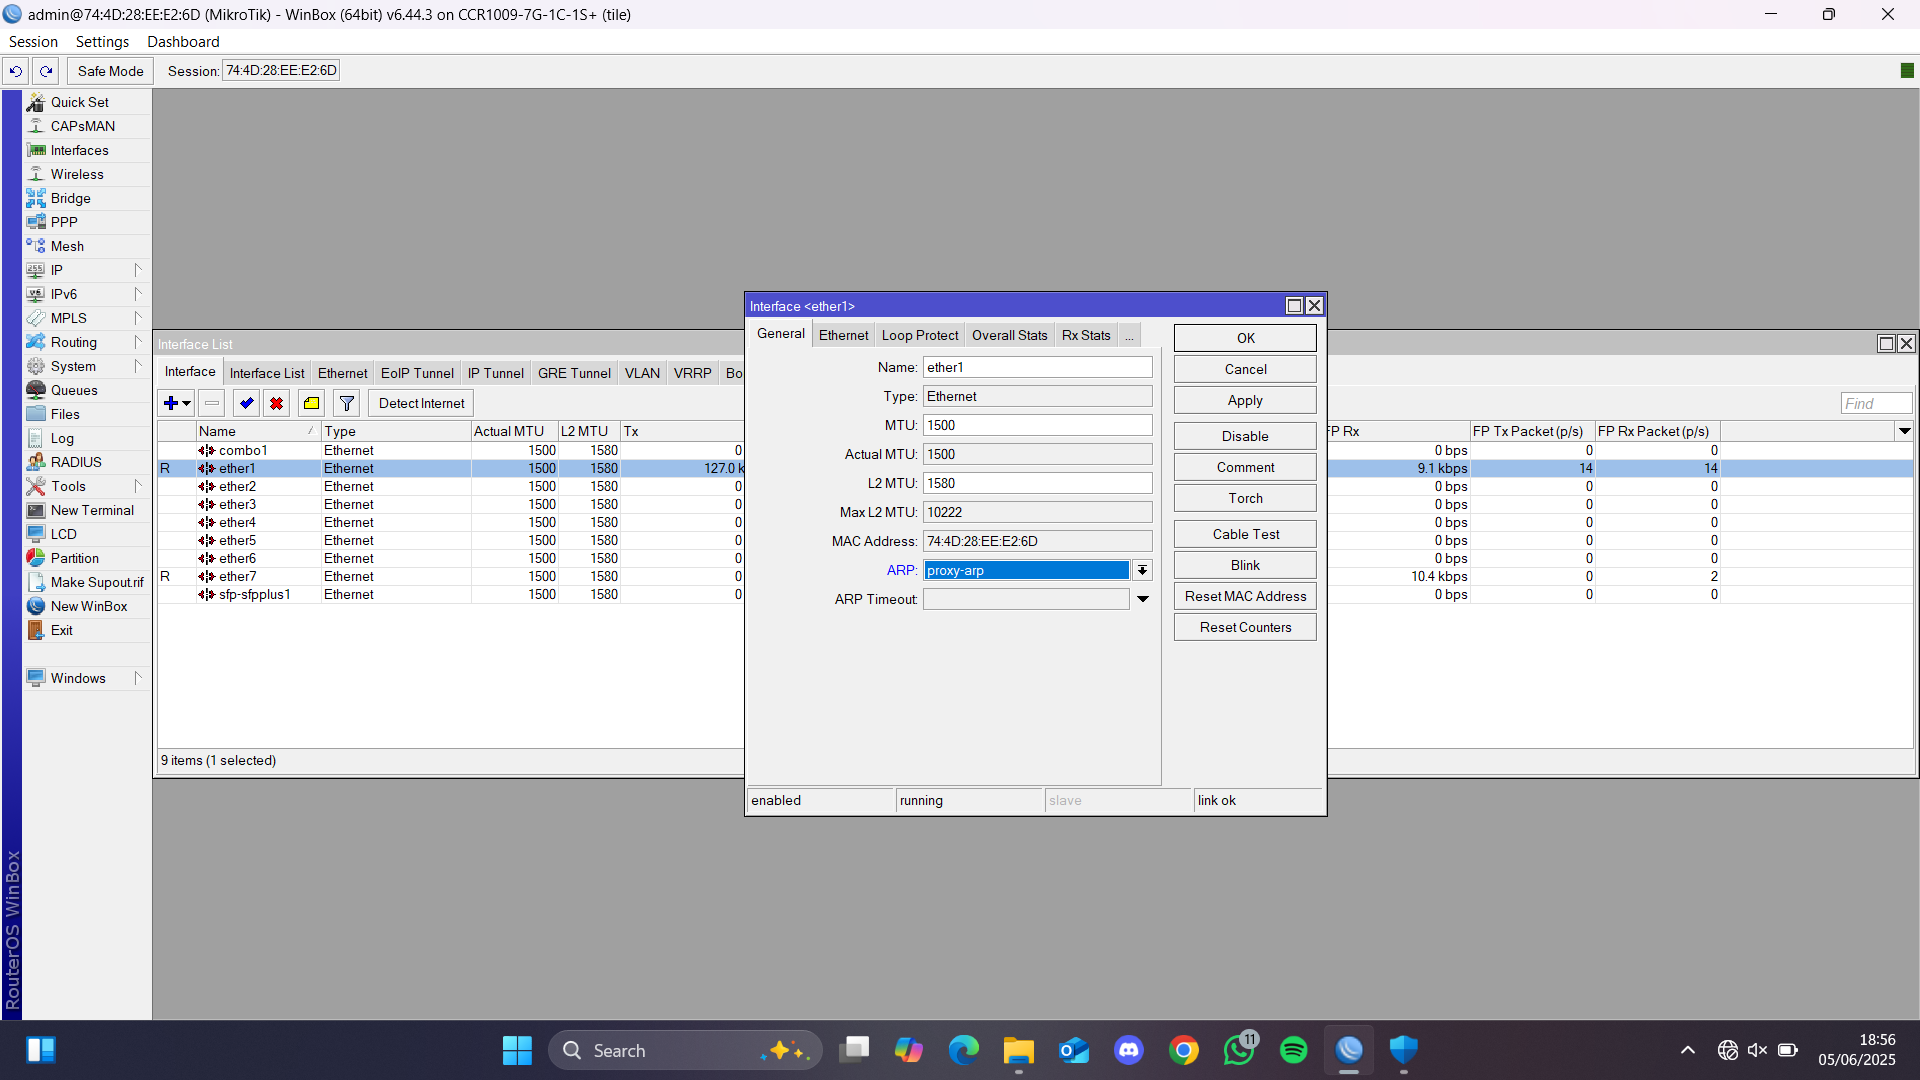
\includegraphics[width=\linewidth]{P5/img/arp.png}
			\caption{Aktifkan Proxy ARP\label{fig:konfigurasiR1}}
		\end{subfigure}
	\end{figure}
	\item Mengaktifkan PPTP server lalu menambahkan secrets dengan konfigurasi nama: mahasiswa, password: praktikum123, service: pptp, local address: 192.168.10.2, remote address: 192.168.10.5.
	\begin{figure}[H]
		\centering
		\begin{subfigure}[b]{0.4\linewidth}
			\centering
			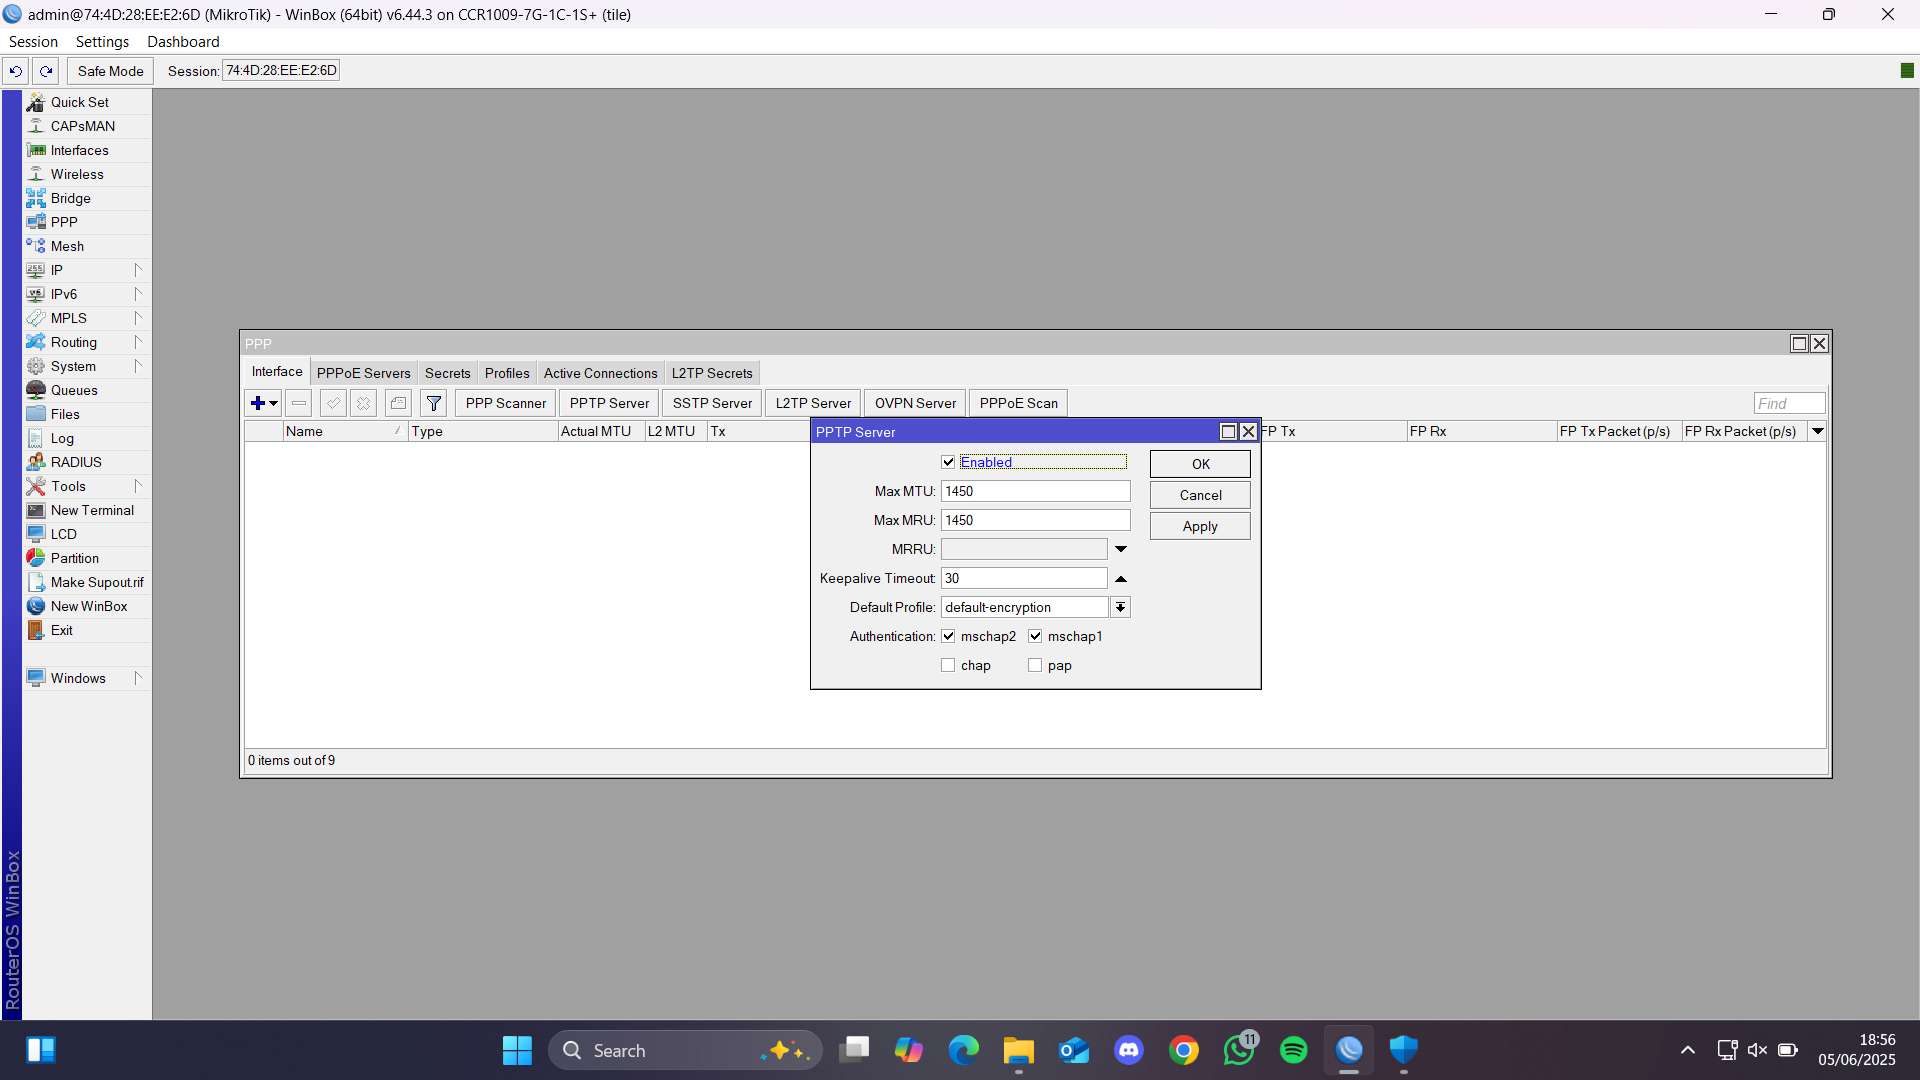
\includegraphics[width=\linewidth]{P5/img/pptp enable.png}
			\caption{Enable PPTP\label{fig:konfigurasiR1}}
		\end{subfigure}
		\begin{subfigure}[b]{0.4\linewidth}
			\centering
			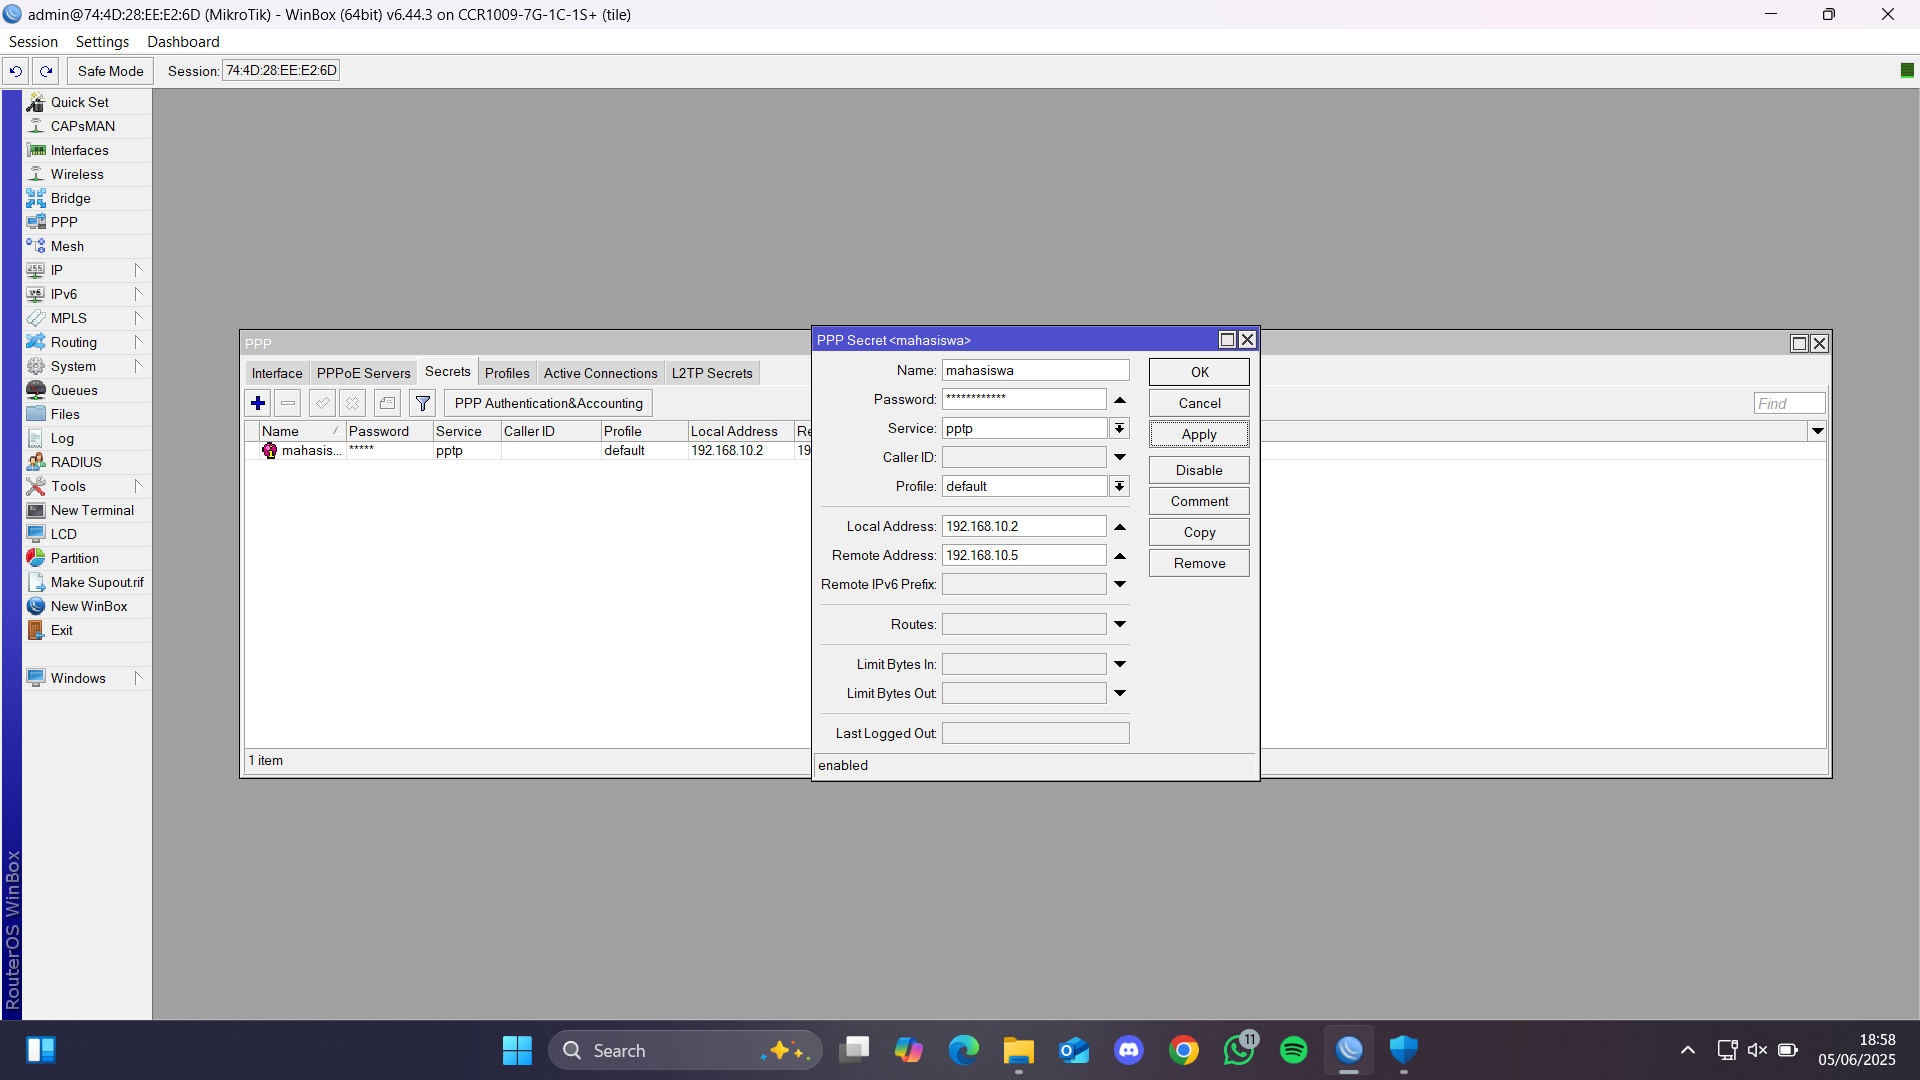
\includegraphics[width=\linewidth]{P5/img/pptp secrets.png}
			\caption{PPTP Secrets\label{fig:konfigurasiR2}}
		\end{subfigure}
		\caption{Konfigurasi PPTP}
		\hspace{1cm}
	\end{figure}
	\item Melakukan konfigurasi VPN PPTP pada laptop B yang terhubung dengan Wi-Fi ITS. Konfigurasi VPN yang digunakan adalah VPN probider: windows, connection name: VPN Router Praktikum, VPN type:
	 Point to Point Tunneling Protocol (PPTP), TYpe of sign-in info: user name and password, user name: mahasiswa, password: praktikum123.
	 \begin{figure}[H]
	 	\centering
	 	\begin{subfigure}[b]{0.4\linewidth}
	 		\centering
	 		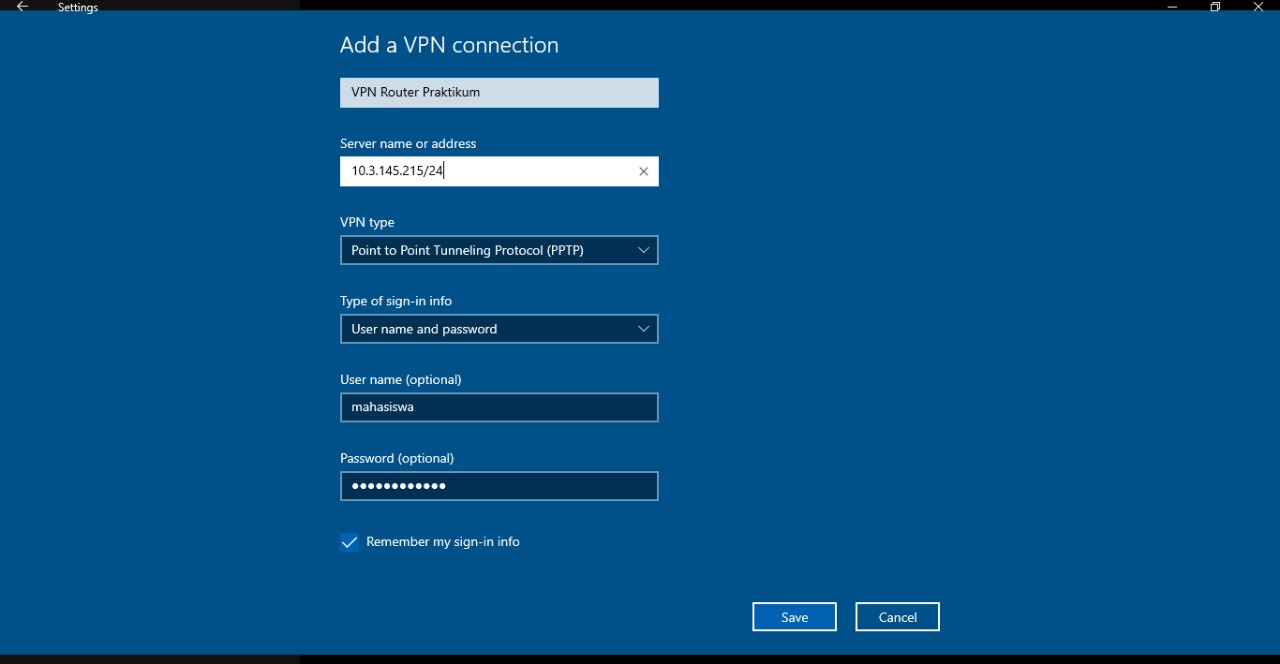
\includegraphics[width=\linewidth]{P5/img/vpn conf.jpg}
	 		\caption{Konfigurasi VPN\label{fig:konfigurasiR1}}
	 	\end{subfigure}
	 	\begin{subfigure}[b]{0.4\linewidth}
	 		\centering
	 		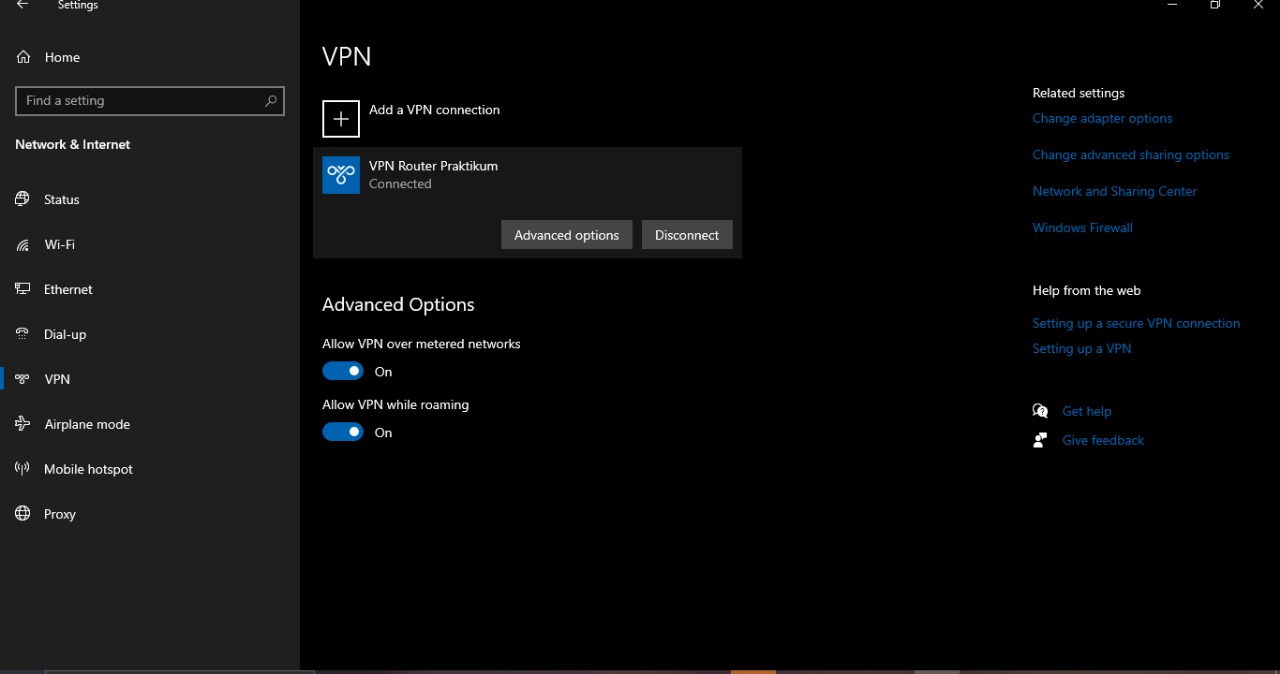
\includegraphics[width=\linewidth]{P5/img/vpn connect.jpg}
	 		\caption{Koneksi VPN\label{fig:konfigurasiR2}}
	 	\end{subfigure}
	 	\caption{Konfigurasi VPN PPTP}
	 	\hspace{1cm}
	 \end{figure}
	\item Memeriksa koneksi VPN dengan menggunakan ipconfig pada powershell/cmd laptop B.
	\item Melakukan uji ping dari laptop B ke router dengan perintah ping 192.168.10.2.
	\item Melakukan uji ping dari laptop B ke laptop A dengan perintah ping 192.168.10.1 (didapatkan dengan menggunakan perintah ipconfig pada laptop A).
	\begin{figure}[H]
		\centering
		\begin{subfigure}[b]{0.4\linewidth}
			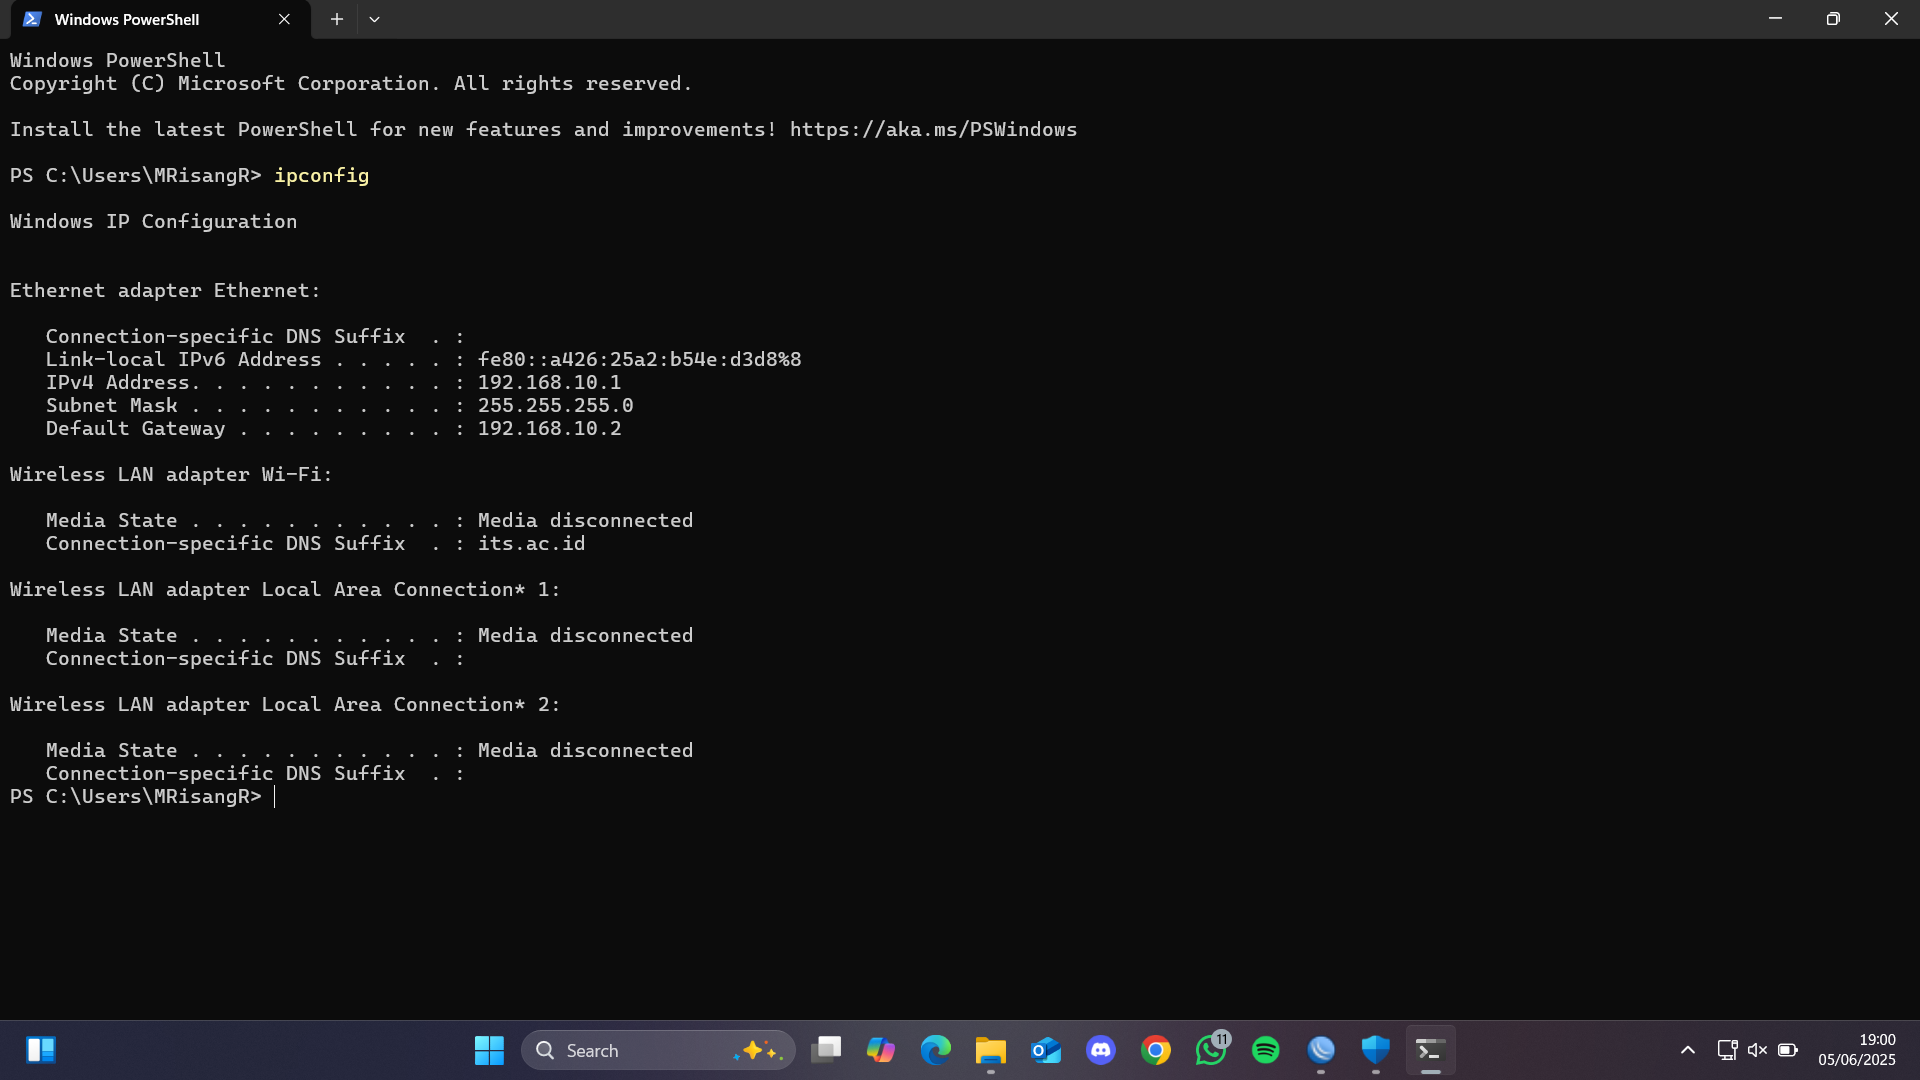
\includegraphics[width=\linewidth]{P5/img/ipconfig laptop.png}
			\caption{ipconfig untuk mengetahui alamat IP laptop A\label{fig:konfigurasiR1}}
		\end{subfigure}
	\end{figure}
\end{enumerate}
\subsection{QoS Pembatasan Bandwidth}
\begin{enumerate}
	\item Membuat aturan simple queue dengan konfigurasi nama: xxx, target: 192.168.10.0/24, max limit (upload): 1M, dan max limit (download): 1M.
	\begin{figure}[H]
		\centering
		\begin{subfigure}[b]{0.4\linewidth}
			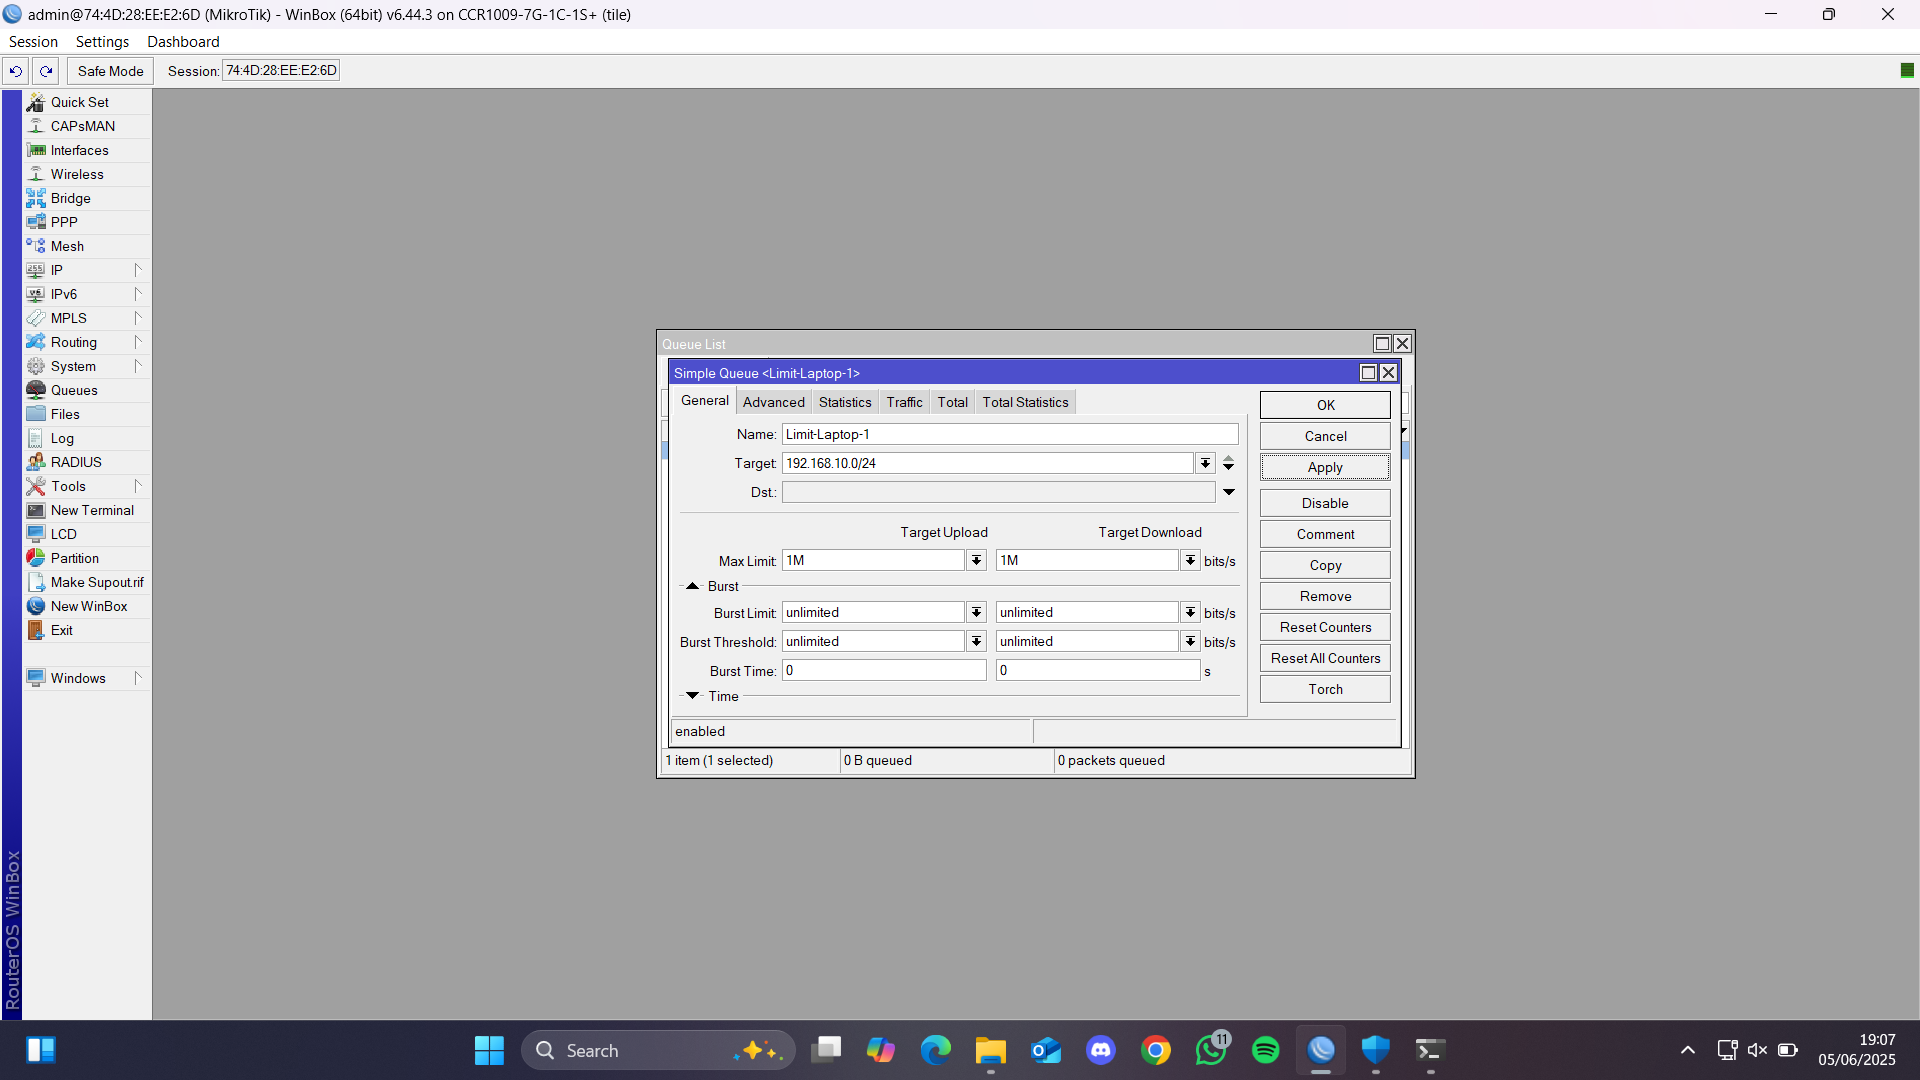
\includegraphics[width=\linewidth]{P5/img/simple q.png}
			\caption{Konfigurasi simple queue\label{fig:konfigurasiR1}}
		\end{subfigure}
	\end{figure}
	\item Memantau penggunaan traffic pada tab Traffic. Diakses dengan double klik pada aturan simple queue yang baru saja dibuat.
	\begin{figure}[H]
		\centering
		\begin{subfigure}[b]{0.4\linewidth}
			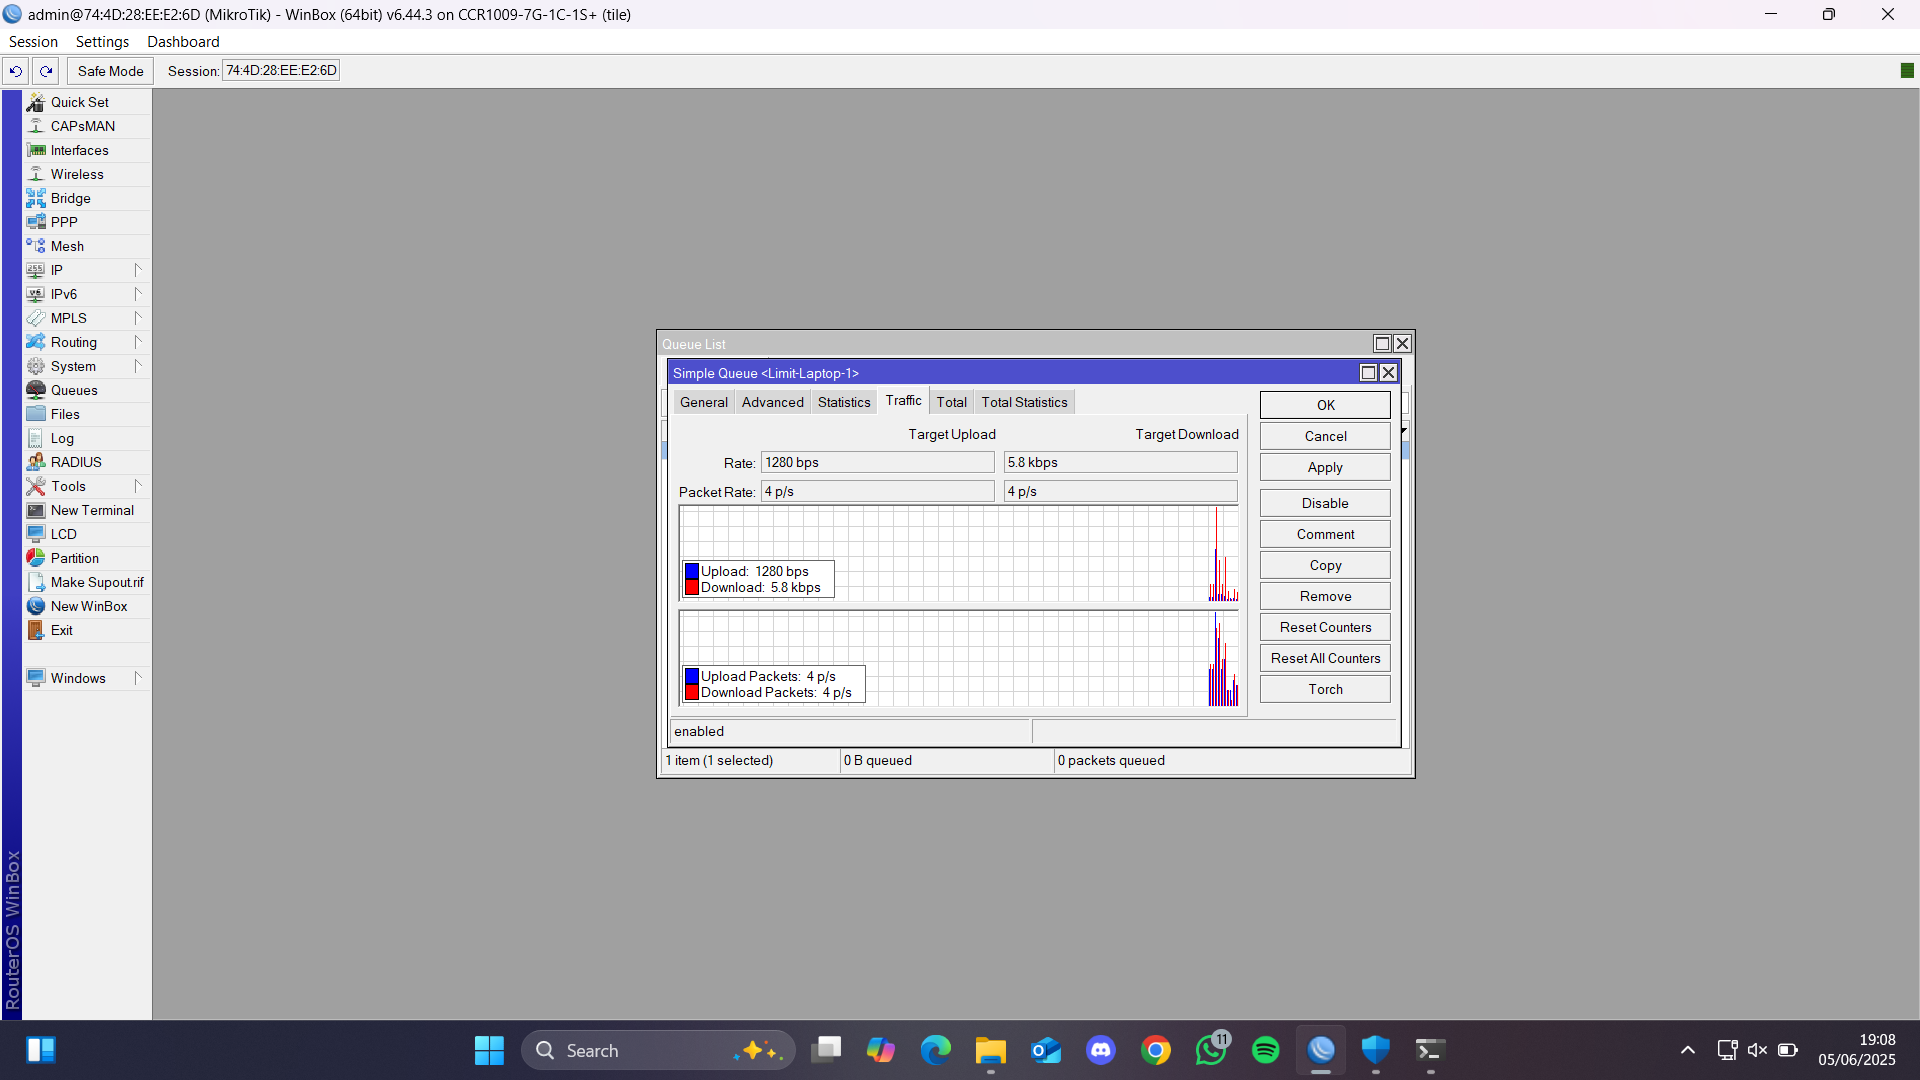
\includegraphics[width=\linewidth]{P5/img/traffic.png}
			\caption{Grafik traffic\label{fig:konfigurasiR1}}
		\end{subfigure}
	\end{figure}
	\item Melakukan pengujian tes kecepatan dengan aturan pembatasan bandwidth nonaktif.
	\item Melakukan pengujian tes kecepatan dengan aturan pembatasan bandwidth aktif.
\end{enumerate}

\section{Analisis Hasil Percobaan}
Pada praktikum ini dilakukan percobaan konfigurasi VPN PPTP dan QoS simple queue untuk pembatasan bandwidth. Secara teori, VPN PPTP memungkinkan dua perangkat yang terhubung ke internet untuk saling berkomunikasi secara privat melalui tunnel yang tidak bisa dilihat oleh pihak lain sehingga seakan komunikasi tersebut terjadi melalui jaringan LAN walaupun kedua perangkat sebenarnya terhubung ke internet. QoS simple queue dapat digunakan untuk membatasi bandwidth bagi jaringan atau host tertentu. Jaringan atau host yang dikenakan pembatasan bandwidth hanya akan dapat mendapatkan kecepatan upload dan download maksimal sesuai yang diatur pada aturan simple queue. Setelah dilaksanakan praktikum, didapatkan hasil bahwa laptop B yang terhubung pada VPN PPTP dapat melakukan ping ke router dan ke laptop A menggunakan alamat IP network 192.168.10.0/24 layaknya melakukan ping pada jaringan LAN walaupiun sebenarnya laptop B hanya terhubung dengan internet melalui Wi-Fi ITS tidak terhubung secara fisik ke router maupun ke laptop A. Kemampuan laptop B untuk melakukan ping ke router dan laptop A menggunakan IP network 192.168.10.0/24 membuktikan bahwa VPN PPTP berhasil.
\begin{figure}[H]
	\centering
	\begin{subfigure}[b]{0.4\linewidth}
		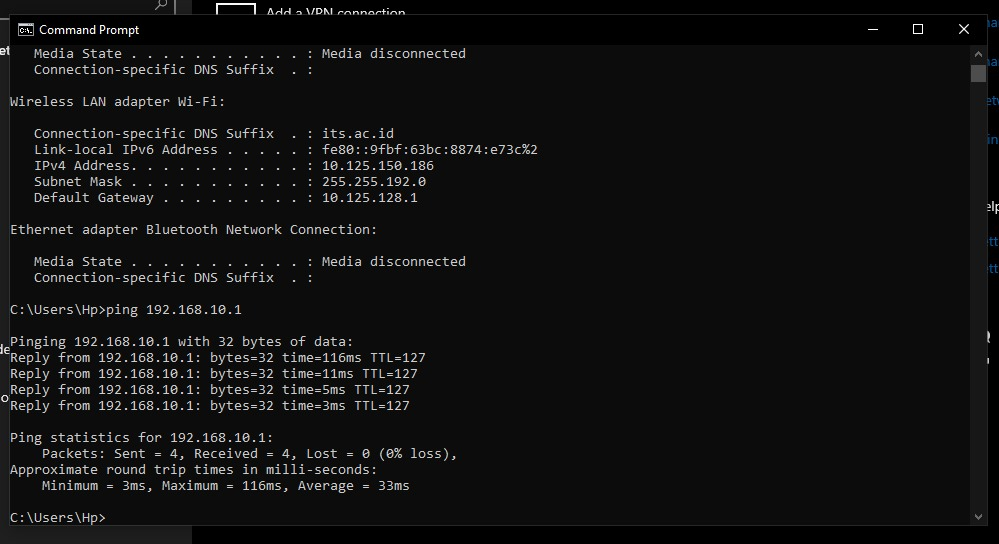
\includegraphics[width=\linewidth]{P5/img/ping laptop.jpg}
		\caption{Hasil ping dari laptop B ke laptop A\label{fig:konfigurasiR1}}
	\end{subfigure}
\end{figure}

Pada percobaan QoS simple queue, didapatkan hasil speedtest tanpa pembatasan bandwidth (aturan simple queue dimatikan) dengan kecepatan download 694,24 Mbps dan upload 807,41 Mbps, namun setelah aturan simple queue diaktifkan didapatkan hasil speedtest dengan kecepatan download 0,65 Mbps dan upload 0,98 Mbps di mana keduanya tidak sampai menyentuh nilai batas maksimum pada aturan simple queue yaitu 1 Mbps. Hasil ini membuktikan bahwa QoS simple queue untuk pembatasan bandwidth berhasil dilakukan.
\begin{figure}[H]
	\centering
	\begin{subfigure}[b]{0.4\linewidth}
		\centering
		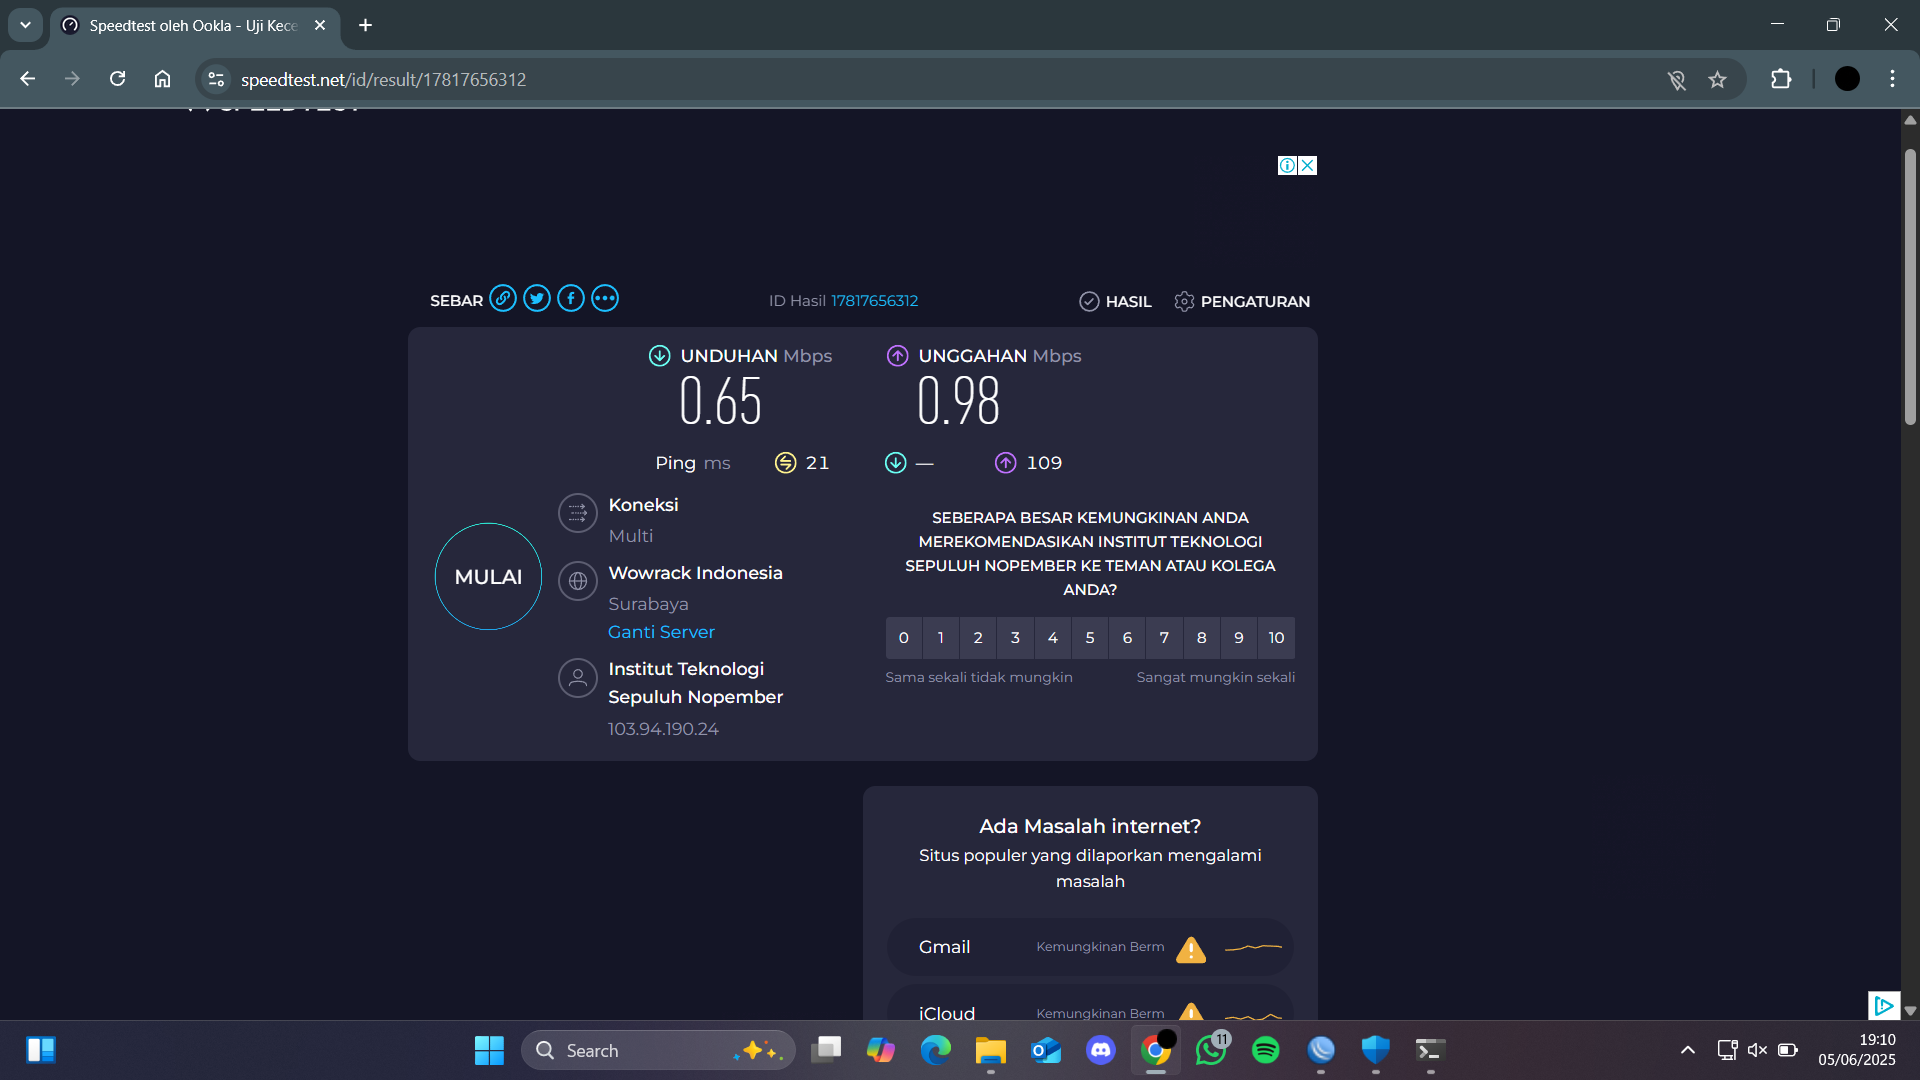
\includegraphics[width=\linewidth]{P5/img/speedtest (1).png}
		\caption{Speedtest tanpa bandwidth limit\label{fig:konfigurasiR1}}
	\end{subfigure}
	\begin{subfigure}[b]{0.4\linewidth}
		\centering
		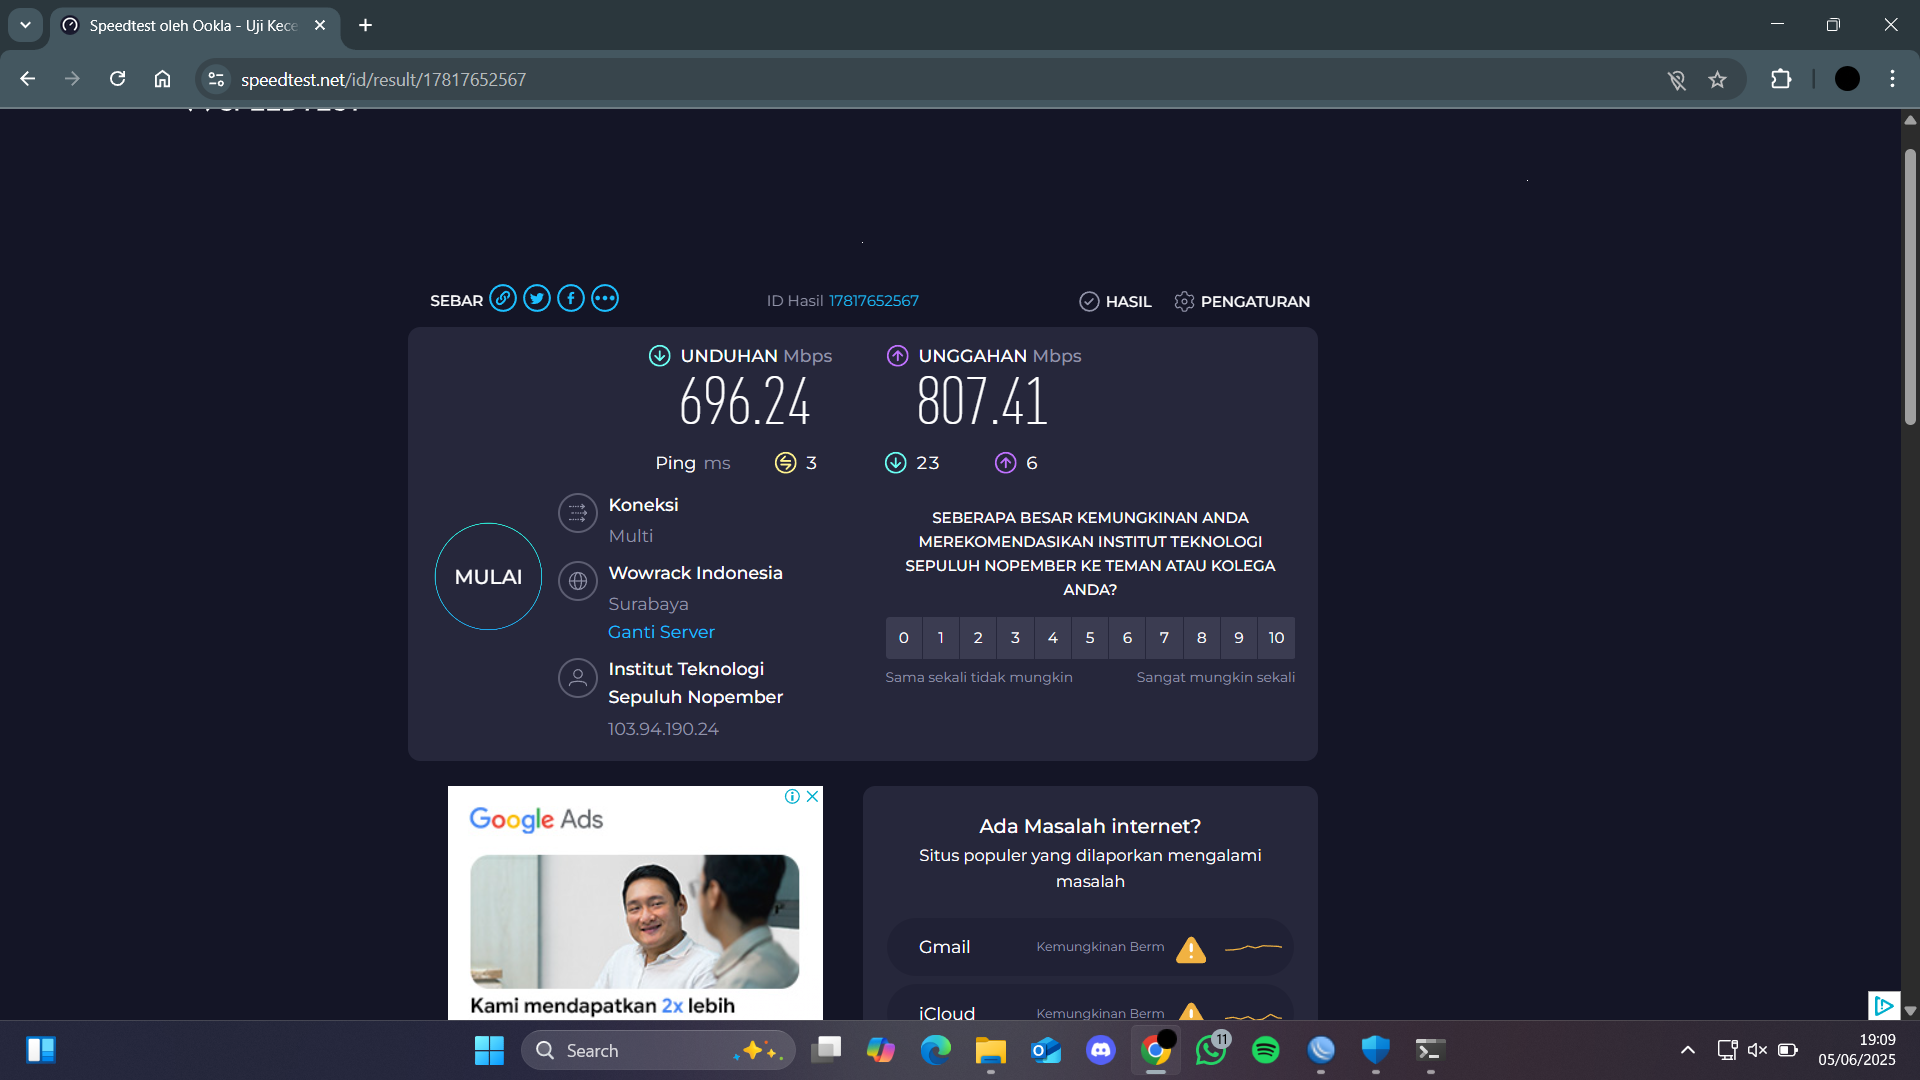
\includegraphics[width=\linewidth]{P5/img/speedtest (2).png}
		\caption{Speedtest dengan bandwidth limit\label{fig:konfigurasiR2}}
	\end{subfigure}
	\caption{Hasil uji kecepatan}
	\hspace{1cm}
\end{figure}

\section{Hasil Tugas Modul}
Berikut merupakan topologi dari jaringan. Koneksi serial antar router digunakan untuk mensimulasikan VPN PPTP karena Cisco Packet Tracer tidak support tunneling PPTP.
\begin{figure}[H]
	\centering
	\begin{subfigure}[b]{0.4\linewidth}
		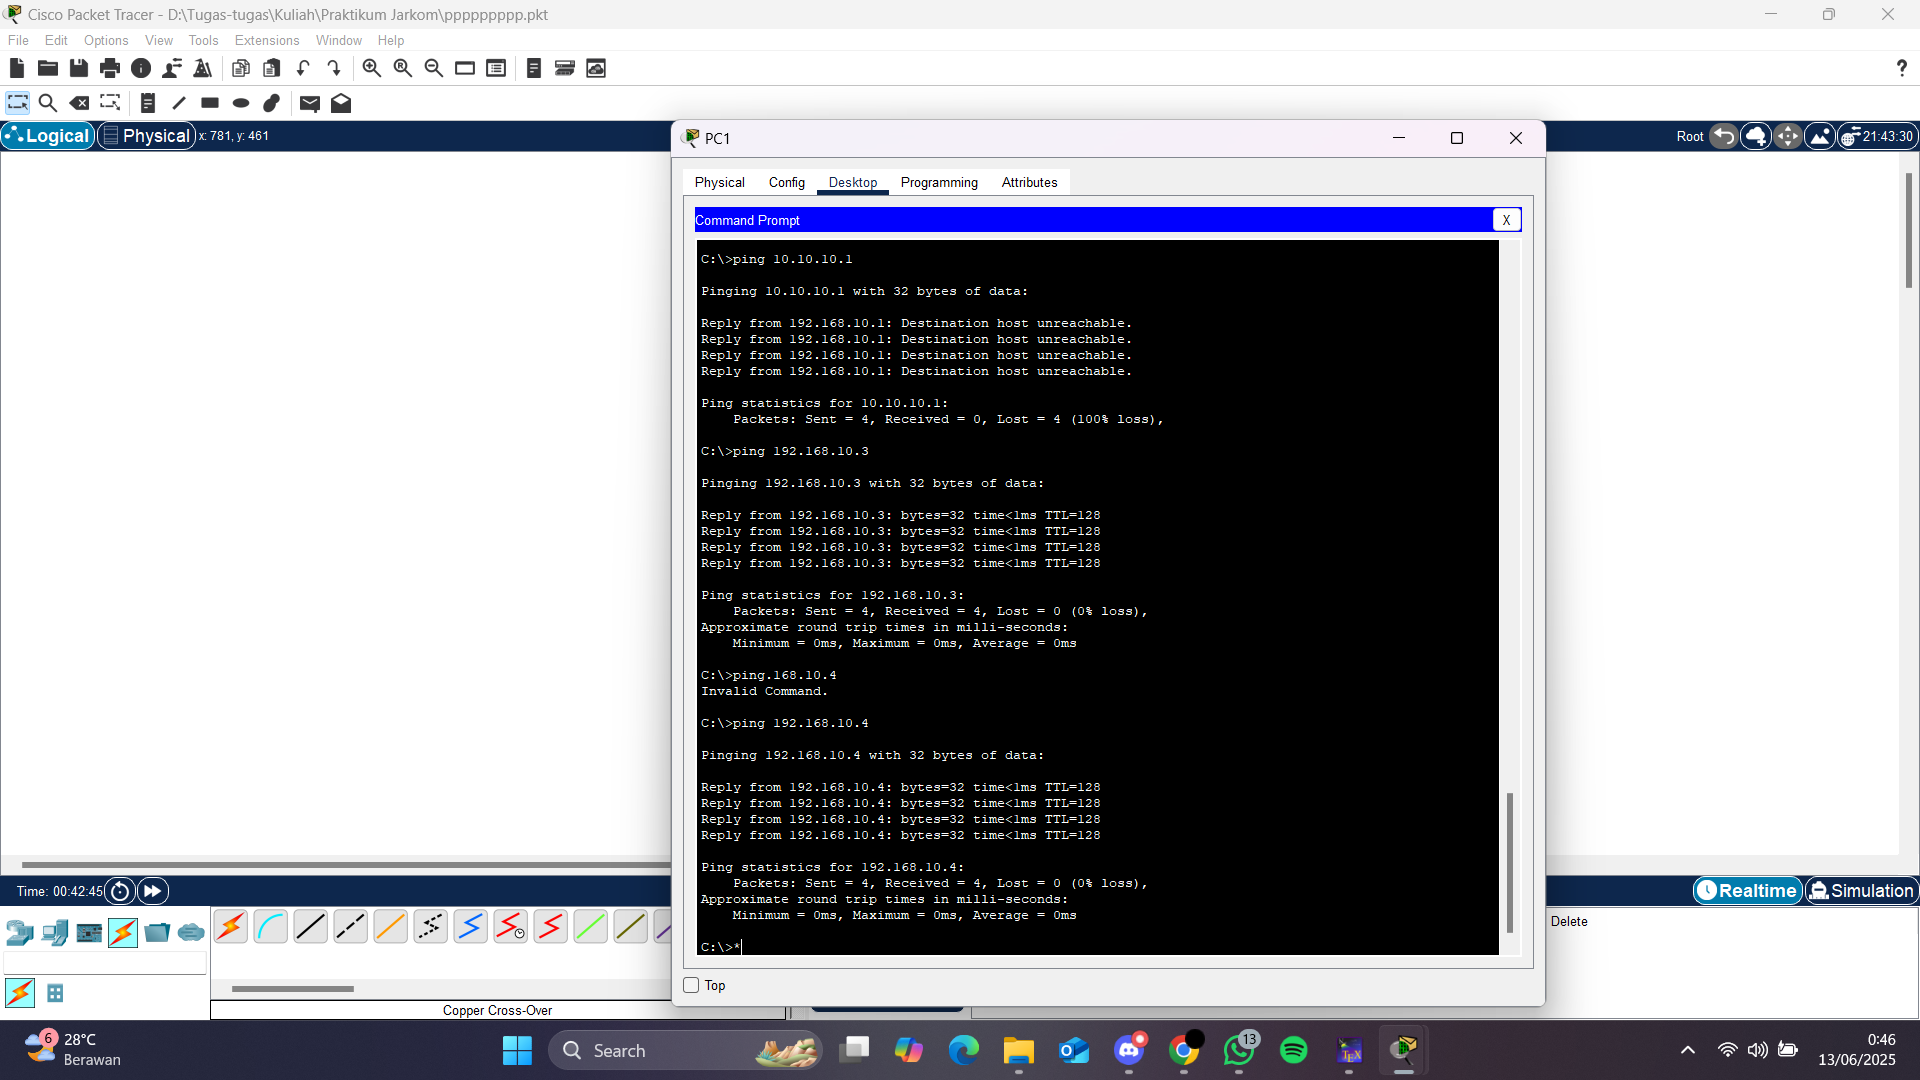
\includegraphics[width=\linewidth]{P5/img/tumod (1).png}
		\caption{Topologi jaringan\label{fig:konfigurasiR1}}
	\end{subfigure}
\end{figure}
Berikut merupakan hasil ping antar PC:
\begin{figure}[H]
	\centering
	\begin{subfigure}[b]{0.4\linewidth}
		\centering
		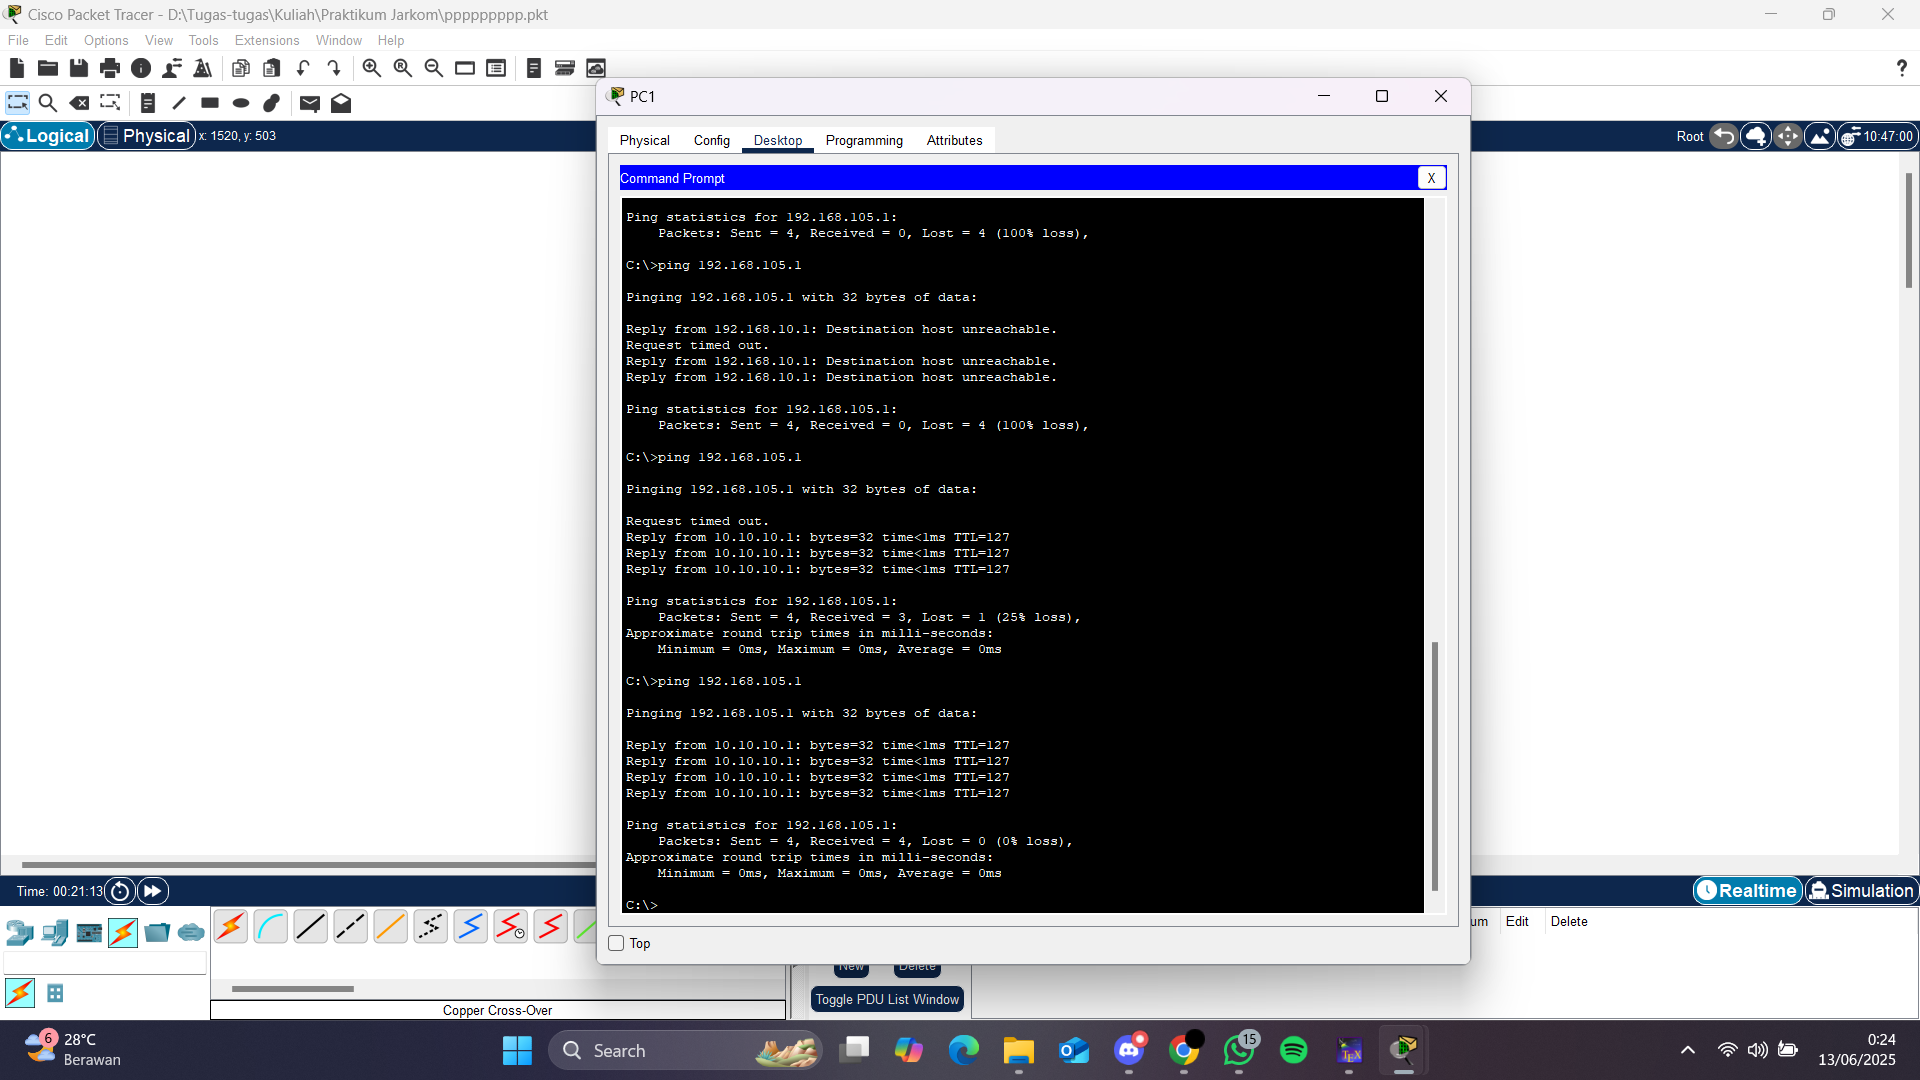
\includegraphics[width=\linewidth]{P5/img/tumod (2).png}
		\caption{Ping dari PC0 ke PC1\label{fig:konfigurasiR1}}
	\end{subfigure}
	\begin{subfigure}[b]{0.4\linewidth}
		\centering
		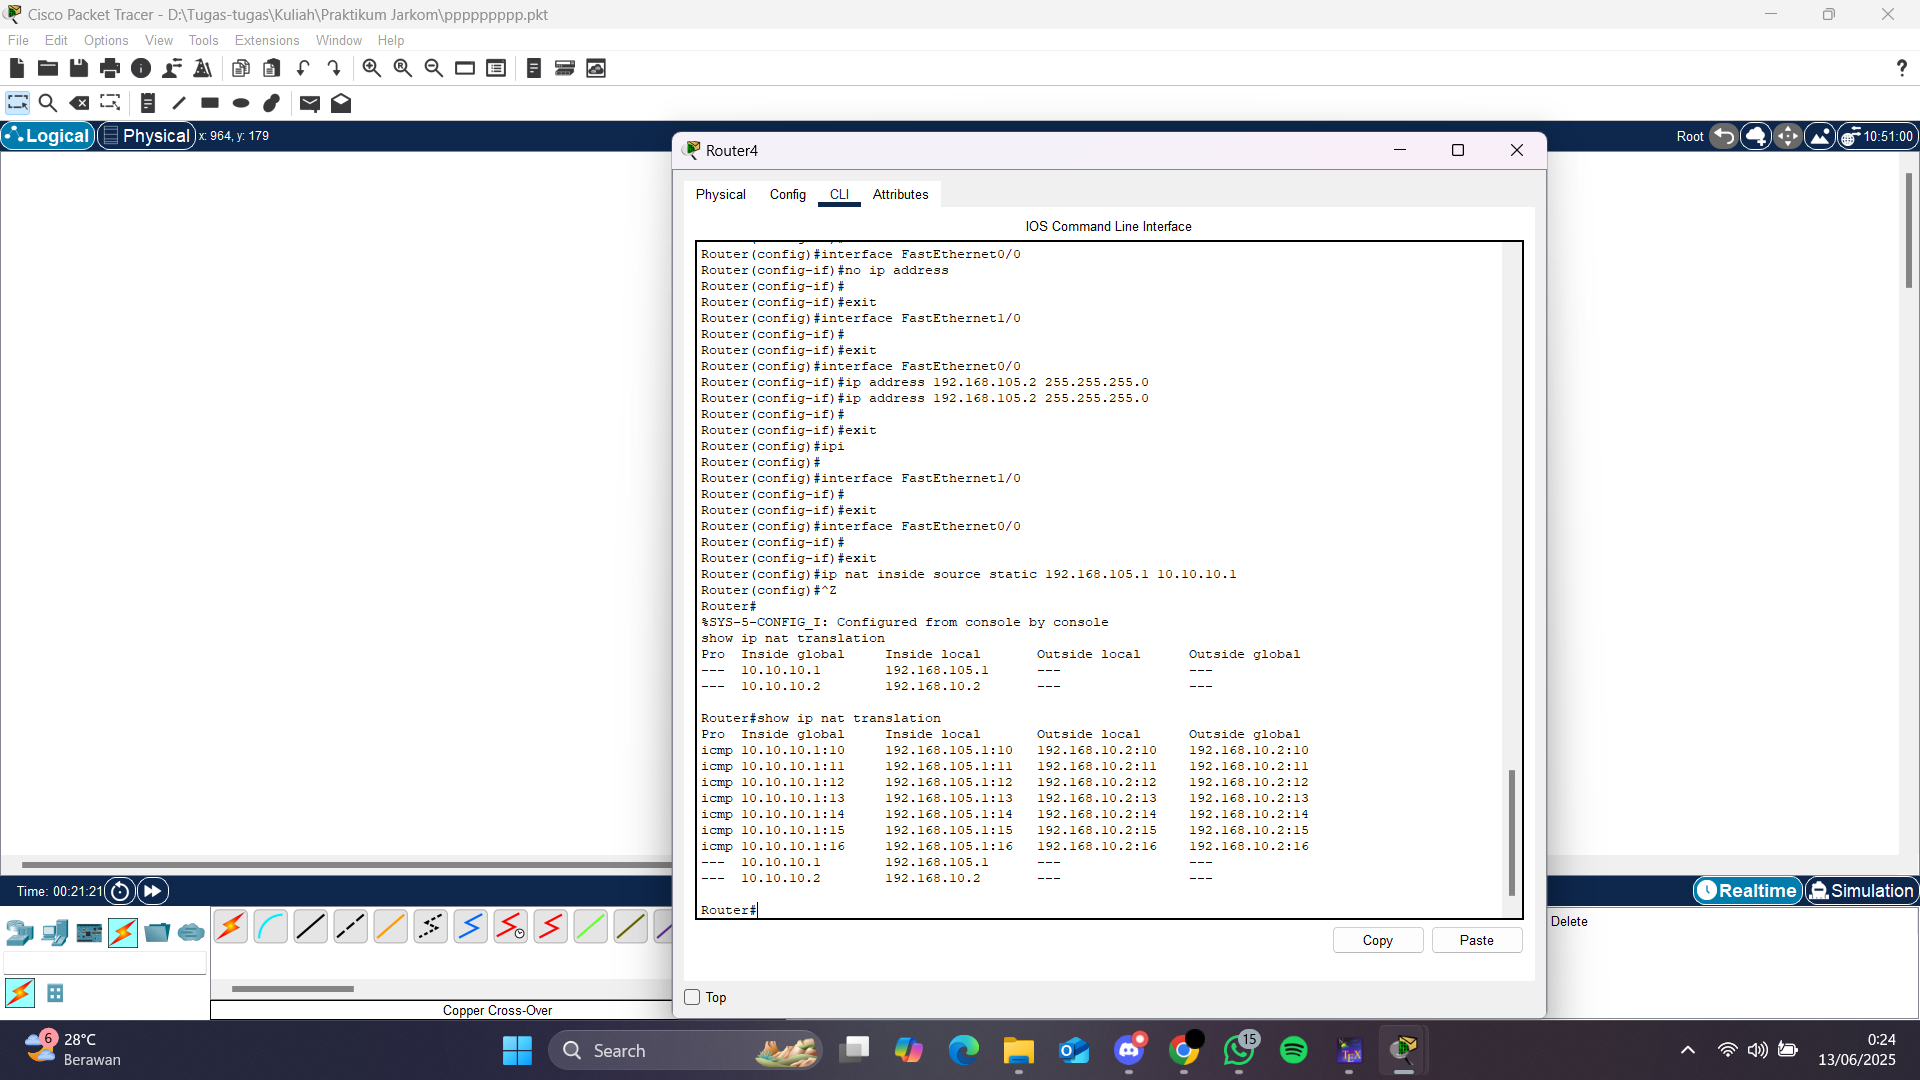
\includegraphics[width=\linewidth]{P5/img/tumod (3).png}
		\caption{Ping dari PC1 ke PC0\label{fig:konfigurasiR2}}
	\end{subfigure}
	\caption{Hasil ping}
	\hspace{1cm}
\end{figure}
PPTP dalam jaringan ini disimulasikan menggunakan koneksi serial antar router karena Cisco Pakcet Tracer tidak support tunneling PPTP. Secara konsep, PPTP berfungsi untuk menghubungkan dua komputer tersebut secara privat melalui tunnel sehingga komunikasi antara dua PC tidak dapat dilihat oleh pihak lain di internet dan kedua PC dapat berkomunikasi seakan keduanya berada dalam jaringan LAN yang sama walaupun sebenarnya keduanya berada dalam jaringan LAN yang berbeda dan terhubung ke satu sama lain melalui internet.

\section{Kesimpulan}
Setelah dilaksanakan praktikum, dapat disimpulkan bahwa VPN PPTP dapat membuat tunnel aman untuk komunikasi pribadi antar perangkat melalui internet sehingga komunikasi tersebut seperti terjadi melalui jaringan LAN walaupun sebenarnya kedua perangkat terhubung dengan satu sama lain melalui internet. QoS simple queue dapat digunakan untuk membatasi bandwidth bagi jaringan atau perangkat tertentu, sehingga dapat dimanfaatkan untuk mengatur pembagian bandwidth yang adil sesuai dengan prioritas pada sebuah jaringan yang memiliki banyak pengguna. Semua hasil dari percobaan yang dilakukan pada praktikum ini sudah cocok dan sesuai dengan teori dan hasil yang diharapkan.

\section{Lampiran}
\subsection{Dokumentasi saat praktikum}
\begin{figure}[H]
	\centering
	\begin{subfigure}[b]{0.4\linewidth}
		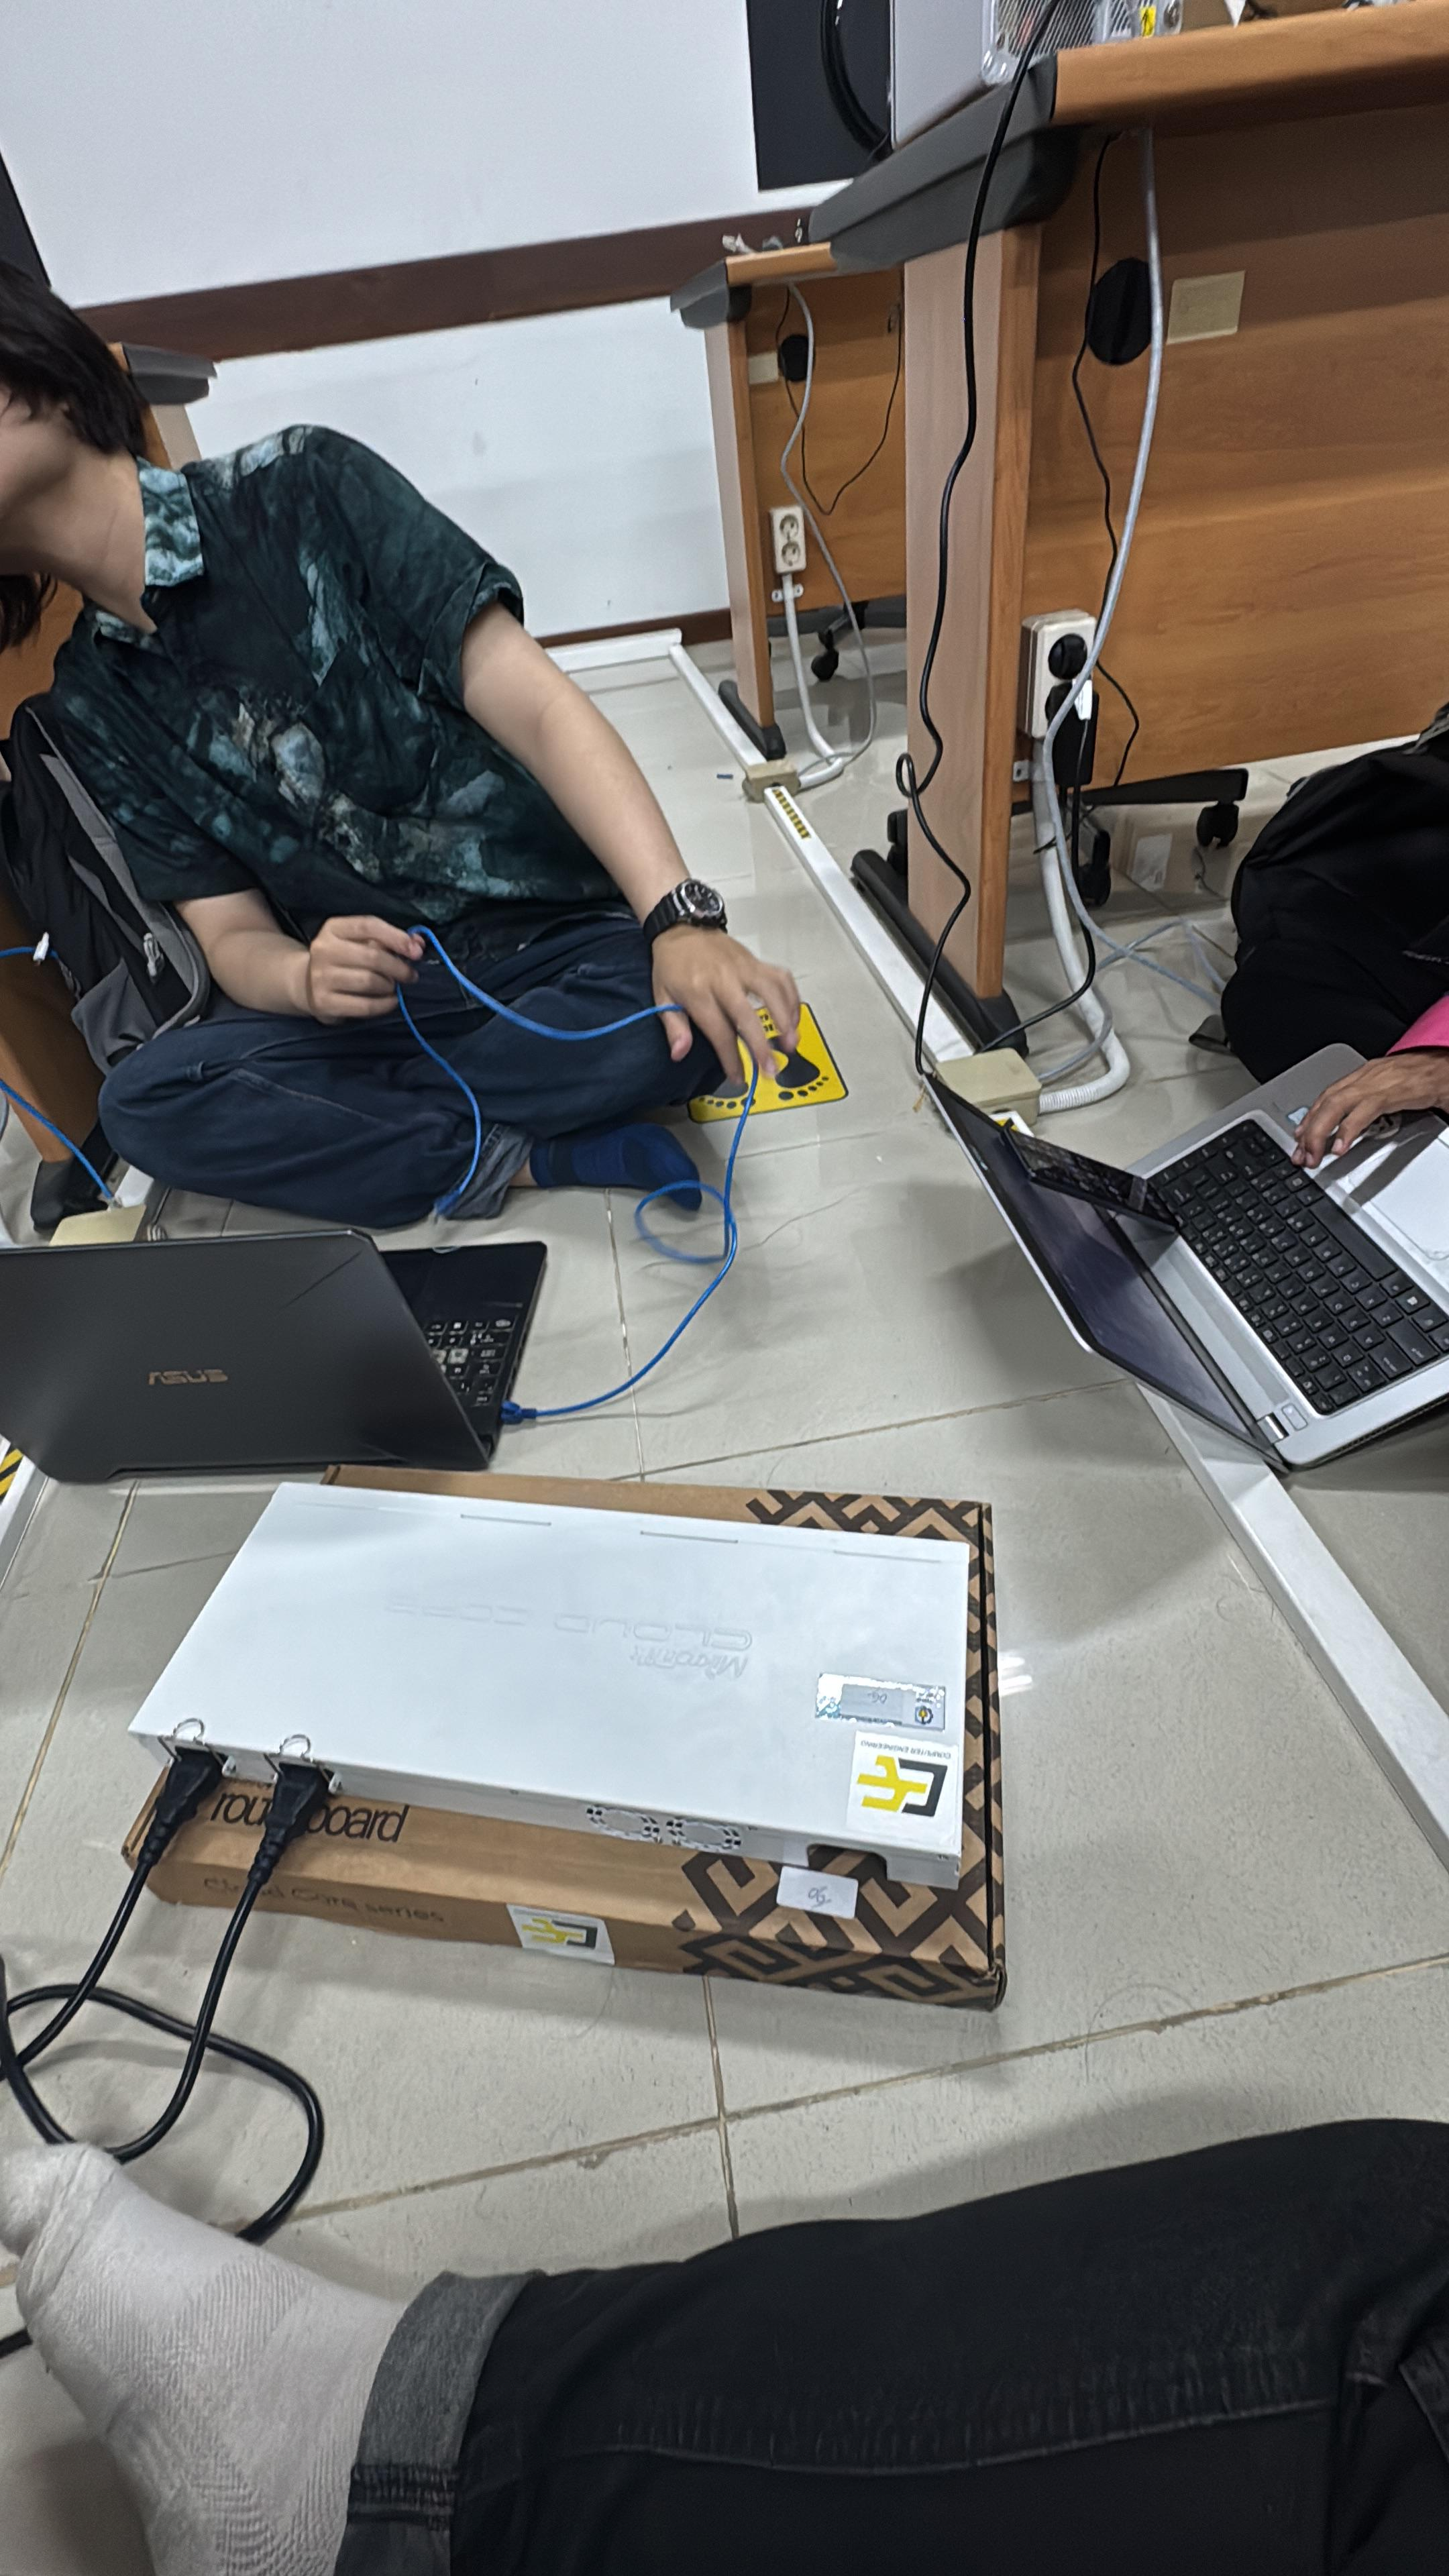
\includegraphics[width=\linewidth]{P5/img/dokum.jpg}
		\caption{Dokumentasi praktikum\label{fig:konfigurasiR1}}
	\end{subfigure}
\end{figure}

\end{document}